\documentclass[]{article}
\makeatletter
\usepackage{lmodern}
\usepackage{comment}
\excludecomment{Answ}
\newcounter{ItemCounter}
\usepackage{listings}
\usepackage{color} %red, green, blue, yellow, cyan, magenta, black, white
\definecolor{mygreen}{RGB}{28,172,0} % color values Red, Green, Blue
\definecolor{mylilas}{RGB}{170,55,241}
\renewcommand\paragraph{\@startsection{paragraph}{4}{\z@}%
            {-2.5ex\@plus -1ex \@minus -.25ex}%
            {1.25ex \@plus .25ex}%
            {\normalfont\normalsize\bfseries}}
\makeatother
\newcommand{\myvec}[1]{\ensuremath{\begin{pmatrix}#1\end{pmatrix}}}
\usepackage{gensymb}
\setcounter{secnumdepth}{4}
\usepackage{amsmath}
%\usepackage{mathtools}
\usepackage{graphicx}
\usepackage{slashed}
\usepackage{lineno}
\usepackage{latexsym}
\usepackage{subfigure}
\usepackage{amssymb}
\newtheorem{thm}{Theorem}[section]
\newtheorem{cor}[thm]{Corollary}
\newtheorem{lem}[thm]{Lemma}
\usepackage[numbers,sort]{natbib}
\usepackage{enumerate}
\newcommand{\bb}{\begin{equation}}
\newcommand{\ee}{\end{equation}}
\newtheorem{defin}{Definition}
\usepackage{multirow}
\usepackage{ctable}
\usepackage{bm}
\usepackage{enumerate}
\newcommand{\D}[2]{\frac{\partial #1}{\partial #2}}
\newcommand{\DD}[2]{\frac{\partial^2 #1}{\partial #2^2}}
\newcommand{\rd}{\text{ d}}
\usepackage{framed}
\newcommand{\see}[1]{(see Figure \ref{#1})}
\newcommand{\fig}[1]{Figure \ref{#1}}
\newcommand{\figs}[2]{figures \ref{#1} and \ref{#2}}
\newcommand{\sect}[1]{Section \ref{#1}}
\newcommand{\app}[1]{Appendix \ref{#1}}
\newcommand{\chap}[1]{Chapter \ref{#1}}
\newcommand{\eqn}[1]{equation \eqref{#1}}
\newcommand{\eqns}[2]{equations \eqref{#1} and \eqref{#2}}
\newcommand{\eqnto}[2]{equations \eqref{#1}-\eqref{#2}}
%\usepackage{authblk}
\usepackage{url}
\usepackage{soul}
\newcommand{\eg}{\emph{e.g.} }
\newcommand{\bn}{\bm{n}}
\newcommand{\bu}{\bm{u}}
\newcommand{\ie}{\emph{i.e.} }
\newcommand{\Chapter}[1]{\chapter{#1}\label{#1}}
\newcommand{\Section}[1]{\section{#1}\label{#1}}
\newcommand{\Subsection}[1]{\subsection{#1}\label{#1}}
\newcommand{\Subsubsection}[1]{\subsubsection{#1}\label{#1}}
\newcommand{\Appendix}[1]{\appendix{#1}\label{#1}}
\usepackage[margin=1.5cm,centering]{geometry}
\usepackage[geometry]{ifsym}
\makeatletter
\newcommand\restr[2]{{% we make the whole thing an ordinary symbol
  \left.\kern-\nulldelimiterspace % automatically resize the bar with \right
  #1 % the function
  \vphantom{\big|} % pretend it's a little taller at normal size
  \right|_{#2} % this is the delimiter
  }}
\def\url@leostyle{%
  \@ifundefined{selectfont}{\def\UrlFont{\sf}}{\def\UrlFont{\small\ttfamily}}}
\makeatother
\urlstyle{leo}
\usepackage{multirow}
\usepackage{blkarray}
\usepackage{soul}
\usepackage{framed}
\usepackage{color}
\usepackage{setspace}
\newcommand{\ttttp}{.24\textwidth}
\newcommand{\tttp}{.32\textwidth}
\newcommand{\ttp}{.45\textwidth}
\newcommand{\tbo}{.6\textwidth}
\newcommand{\tp}{\textwidth}
 \usepackage[T1]{fontenc}
\usepackage[utf8]{inputenc}
\usepackage{authblk}
 \renewcommand{\l}{\left(}
\renewcommand{\r}{\right)}
%\begin{figure}[h!!!tb]
%\centering
%\subfigure[\label{Godzilla}]{\includegraphics[height=0.35\textwidth]{./Pictures/Godzilla_final_bw.png}}
%\subfigure[\label{Jaeger}]{\includegraphics[height=0.35\textwidth]{./Pictures/Jaeger_finish_bw.png}}
%\caption{\label{Monsters} The two types of monster we are going to consider are: (a) the naturally occurring Kaijus and (b) the man-made Jaegers.}
%\end{figure}


\begin{document}

\lstset{language=Matlab,%
    %basicstyle=\color{red},
    breaklines=true,%
    morekeywords={matlab2tikz},
    keywordstyle=\color{blue},%
    morekeywords=[2]{1}, keywordstyle=[2]{\color{black}},
    identifierstyle=\color{black},%
    stringstyle=\color{mylilas},
    commentstyle=\color{mygreen},%
    showstringspaces=false,%without this there will be a symbol in the places where there is a space
    numbers=left,%
    numberstyle={\tiny \color{black}},% size of the numbers
    numbersep=9pt, % this defines how far the numbers are from the text
    emph=[1]{for,end,break},emphstyle=[1]\color{red}, %some words to emphasise
    %emph=[2]{word1,word2}, emphstyle=[2]{style},    
}


\title{Problem sheet 4}
\author{Thomas E. Woolley\\Last edited on:}
\maketitle
\section{Lotka-Volterra equations}\label{Lotka-Volterra equations}
Data on the number of Canadian lynx and snowshoe hair pelts traded where collected by the  Hudson Bay trading company\footnote{Caution about the data: I have not been able to verify this data, but this is the data (or rather the graph) that is always cited. This particular set of data came from scanning in the graph from Odum's "Fundamentals of Ecology", p. 191 which is often cited. Odum says that his graph is taken from MacLulich's "Fluctuations in the numbers of varying hare", 1937, which is not widely available. Some authors caution that this data is actually a composition of several time series, and should probably not be analysed as a whole, and that some of the lynx data was actually missing. It is said that the data was collected from Hudson's Bay historical records, and does not reflect animal populations, but rather the number of pelts turned in for trading (a large number of which came from Native Americans- mentioned because there were some medical outbreaks during these years which could account for skewed data). The data are presented here with these cautions. }. The data are presented in \fig{Lynx_hare} and has been used as a proxy for population data.
\begin{figure}[h!!!tb]
\centering
\subfigure[]{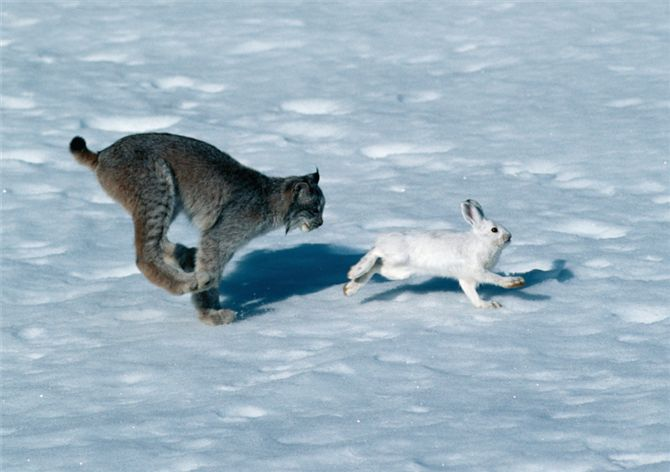
\includegraphics[height=\tttp]{../../Pictures/Lynx_chasing_hare.jpeg}}
\subfigure[\label{Lynx_hare}]{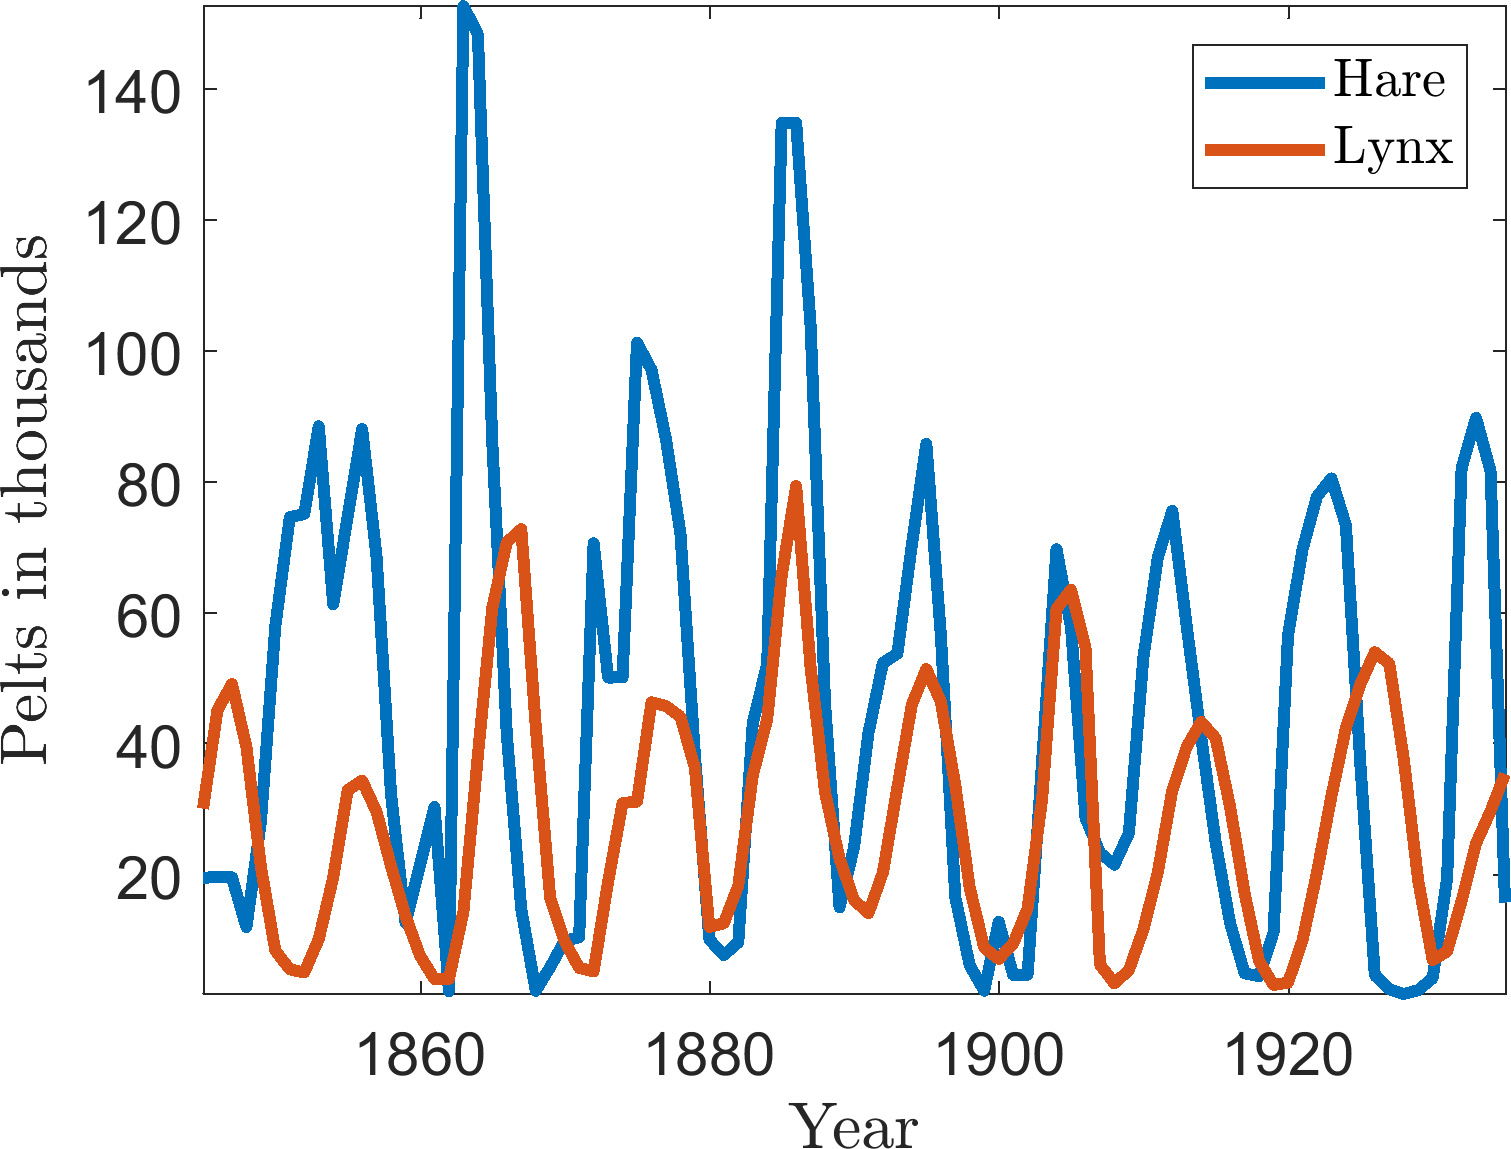
\includegraphics[height=\tttp]{../../Pictures/Lynx_hare.png}}
\caption{ (a) Lynx and hare in action. (b) Number of pelts recorded over time.}
\end{figure}
In this question we consider a mathematical model that has been suggested to describe the features seen in the data. Specifically, it is a predator-prey interaction model called the Lotka-Volterra model. Let $L$ be the lynx population and $H$ be the hare population. The interaction equations are 
\bb
\underbrace{H\stackrel{k_1}{\rightarrow}2H}_{\textrm{Hares reproduce.}}, \quad \underbrace{H+L\stackrel{k_2}{\rightarrow}2L}_{\textrm{Lynx reproduce through predation.}}, \quad \underbrace{L\stackrel{k_3}{\rightarrow}\slashed{0}}_{\textrm{Lynx die out.}}.
\ee
\begin{enumerate}
\item Describe two features seen in the population data of \fig{Lynx_hare}.
\item Name two troubling assumptions behind the Lotka-Volterra interaction equations and suggest how they could be fixed.
\item Write down the ODEs representing the interaction system.
\item Let $u$ and $v$ be non-dimensional variables of the hare and lynx, respectively. Non-dimensionalise the system to produce a system of the form:
\begin{align}
\dot{u}&=u-uv,\label{LV1}\\
\dot{v}&=\alpha(uv-v)\label{LV2},
\end{align}
where the time derivative is with respect to some non-dimensionalised time.

Provide the dimensional scales of the population (i.e. $[L]$, $[H]$ and $[t]$) as well as the definition of $\alpha$. Note, that you are not required to show that $[L]$ and $[H]$ have the right dimension and $\alpha$ is dimensionless, but it is a good way to check your working.
\item What are the steady states?
\item What is the linear stability of the states?
\item Consider
\bb
\frac{\rd u}{\rd v}=\frac{\dot{u}}{\dot{v}}.\label{LV_solvable}
\ee
Show that \eqn{LV_solvable} can be directly integrated to show that the populations must satisfy the constraint
\bb
\l\frac{e^{v}}{v}\r\l\frac{e^{u}}{u}\r^\alpha=e^{C},\label{LV_conserved}
\ee
where $C$ is a constant of integration that depends on the initial conditions. (Hint: rearrange $\rd u/\rd v$ such that one side contains all $u$ terms and the other contains all $v$ terms).
\end{enumerate}
\begin{Answ}
\subsection{Answers}
\subsubsection{}
The populations oscillate. A rise in prey comes before a rise in predator. Other sensible comments are allowed.
\subsubsection{}
\begin{enumerate}[(a)]
\item Prey does not die naturally, a prey death rate could be included.
\item Predator and prey do not need partners to reproduce, such reproduction equations could be included.
\item Predation is a one to one transference, usually more prey are needed to produce enough energy to provide a new predator generation. Instead of producing two lynx we could rewrite the predation equation to give $1+\epsilon$ predators.
\item Other assumptions and fixes are available.
\end{enumerate}
\subsubsection{}
\begin{align}
\dot{H}&=k_1H-k_2HL,\\
\dot{L}&=k_2HL-k_3L.
\end{align}
\subsubsection{}
Let $H=[H]u$, $L=[L]v$, $t=[t]\tau$, the appropriate scales are then:
\bb
[H]=\frac{k_3}{k_2},\quad [L]=\frac{k_1}{k_2},\quad [t]=\frac{1}{k_1}
\ee
and $\alpha=k_3/k_1$.
\subsubsection{}
The steady states are $(0,0)$ and $(1,1)$.
\subsubsection{}
The Jacobian of the system is
\bb
J(u,v)=\left[ {\begin{array}{cc}
   1-v & -u \\
   \alpha v & \alpha(u-1) \\
  \end{array} } \right].
\ee
For (0,0)
\bb
J(0,0)=\left[ {\begin{array}{cc}
   1 & 0 \\
   0 & -\alpha \\
  \end{array} } \right],
\ee
the eigenvalues are, thus, $\lambda=1>0$ and $-\alpha<0$. Hence, (0,0) is a saddle point.

For (1,1)
\bb
J(0,0)=\left[ {\begin{array}{cc}
   0 & -1 \\
   \alpha & 0 \\
  \end{array} } \right],
\ee
the eigenvalues are, thus, $\lambda=\pm\sqrt{-\alpha}$, which are purely imaginary. Hence (1,1) is a centre.
\subsubsection{}
\bb
\frac{\rd u}{\rd v}=\frac{u\l 1-v\r}{\alpha v\l u-1\r}
\ee
which can reformulated to be
\bb
\int^u_{u_0}\frac{\alpha(u-1)}{u}\rd u=\int^v_{v_0}\frac{1-v}{v}\rd v,
\ee
from which we can derive
\bb
\alpha(u-\log(u))-\alpha(u_0-\log(u_0))=(\log(v)-v)-(\log(v_0)-v_0),
\ee
which can be rearranged to be
\bb
\alpha(u-\log(u))+v-\log(v)=\alpha(u_0-\log(u_0))+v_0-\log(v_0).
\ee
Exponentiating both sides of the equation we get
\bb
e^{u\alpha}u^{-\alpha}e^{v}v^{-1}=e^{\alpha(u_0-\log(u_0))+v_0-\log(v_0)},
\ee
which can finally be rearranged to produce
\bb
\l\frac{e^{v}}{v}\r\l\frac{e^{u}}{u}\r^\alpha=e^{C},\label{Conserved}
\ee
where $C=\alpha(u_0-\log(u_0))+v_0-\log(v_0)$.
\end{Answ}
\section{Computer simulation}
Let $\alpha=1/2$ and simulate \eqns{LV1}{LV2}. Plot the results in the $(u,v)$ plane along with \eqn{LV_conserved}. Note you will have to choose appropriate initial conditions, specify $C$ in terms of these initial conditions and use an implicit plotting algorithm such as \texttt{fimplicit} in MatLab.
\begin{enumerate}
\item Vary the initial conditions, what do you notice?
\item Do your discoveries accord with the results from question \ref{Lotka-Volterra equations}?
\item Now consider the plot of $(t,u)$ and $(t,v)$. Do the simulated curves match the data seen in \fig{Lynx_hare}?
\end{enumerate}
\begin{Answ}
\subsection{Answers}
\subsubsection{}
The simulations can be seen in \fig{LV_sims}.
\begin{figure}[h!!!tb]
\centering
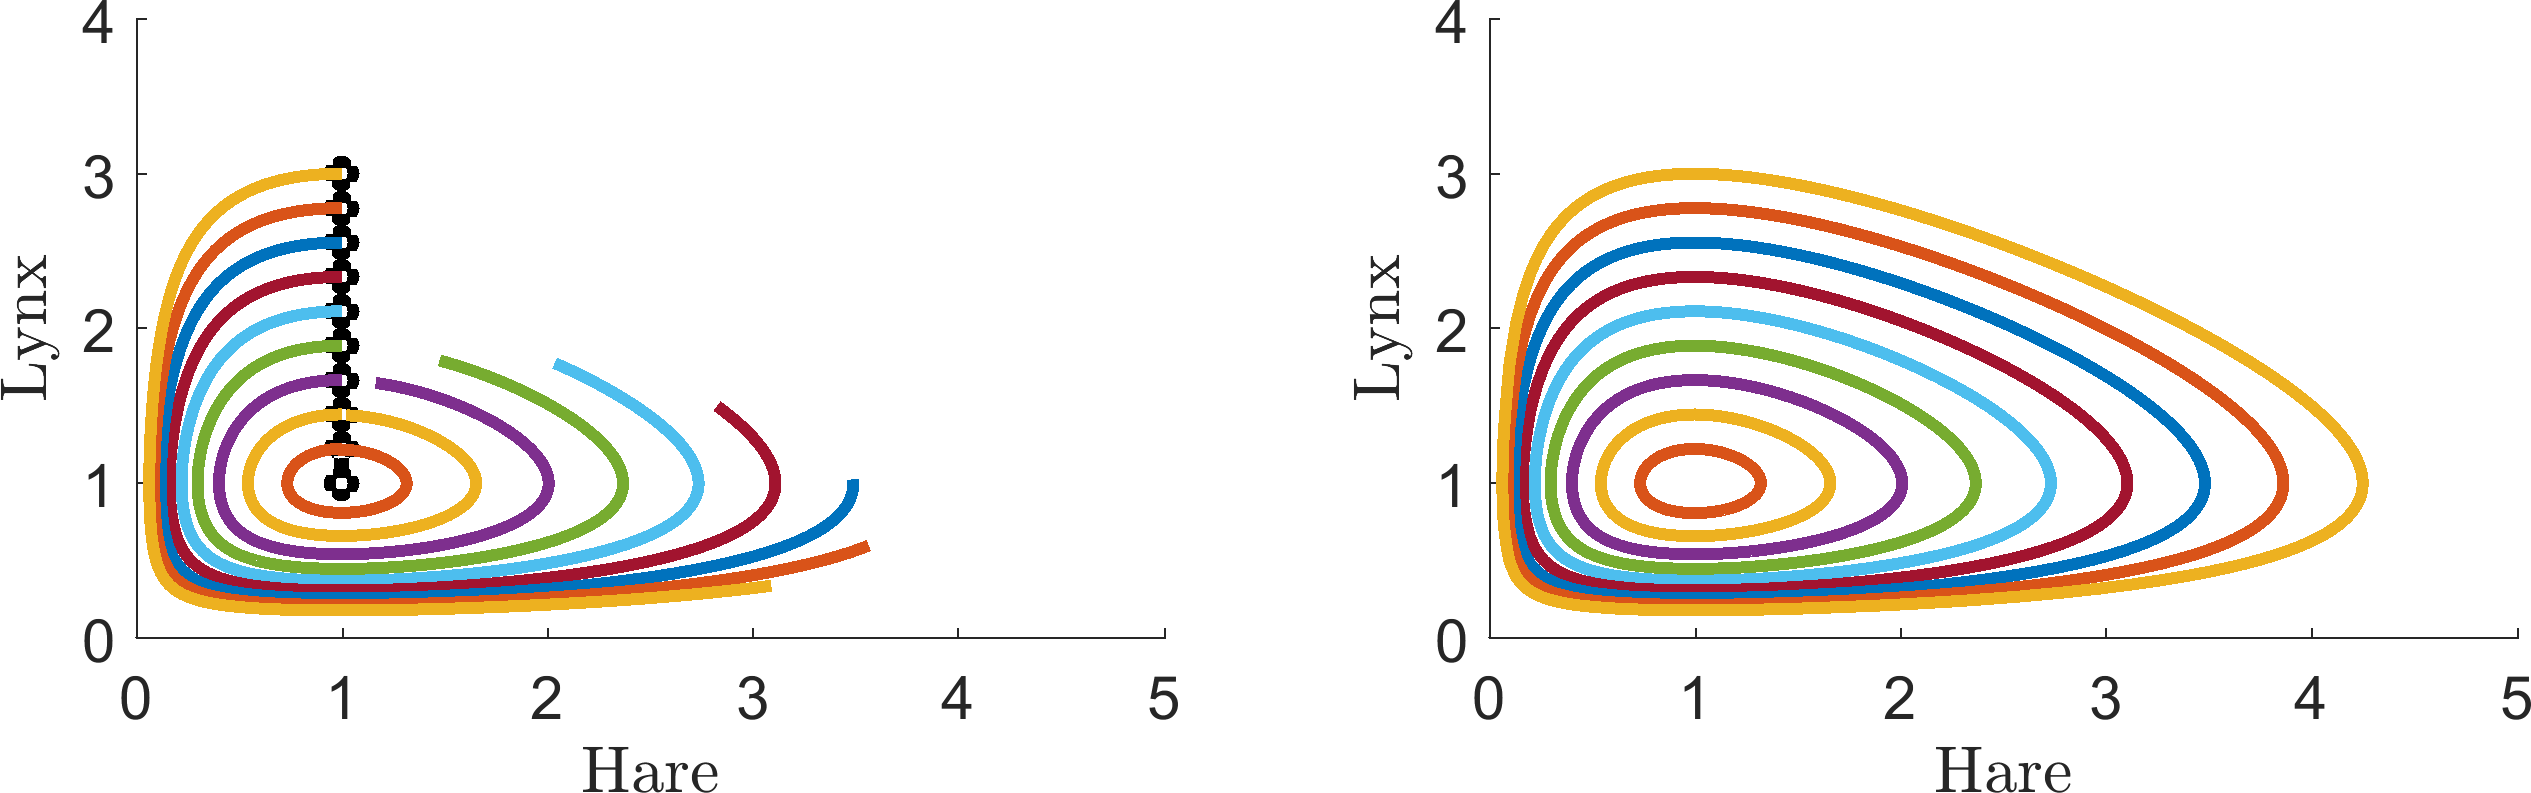
\includegraphics[width=\textwidth]{../../Pictures/LV_sims.png}
\caption{Left: simulation of \eqns{LV1}{LV2}. The black points illustrate the initial condition, the trajectories are spiralling anticlockwise. Right: Simulation of \eqn{Conserved} with the same initial conditions as in the left image.\label{LV_sims}}
\end{figure}
Different initial conditions cause the trajectory to be on different parallel oscillatory trajectories. The trajectories are exactly matched by the curves given by \eqn{Conserved}. Larger initial conditions have a longer period.

\subsubsection{}
The simulations in \fig{LV_sims} exactly match the linearised stability solution suggesting that (1,1) is a centre. However, the simulations illustrate that this is a global phenomenon, in that all trajectories periodically oscillate around (1,1).
\subsubsection{}
The time course simulation in \fig{LV_time_sims} illustrate that the trajectories do have similar traits of periodic oscillations and that growth in the lynx population lags behind growth in the  hare population.
\begin{figure}[h!!!tb]
\centering
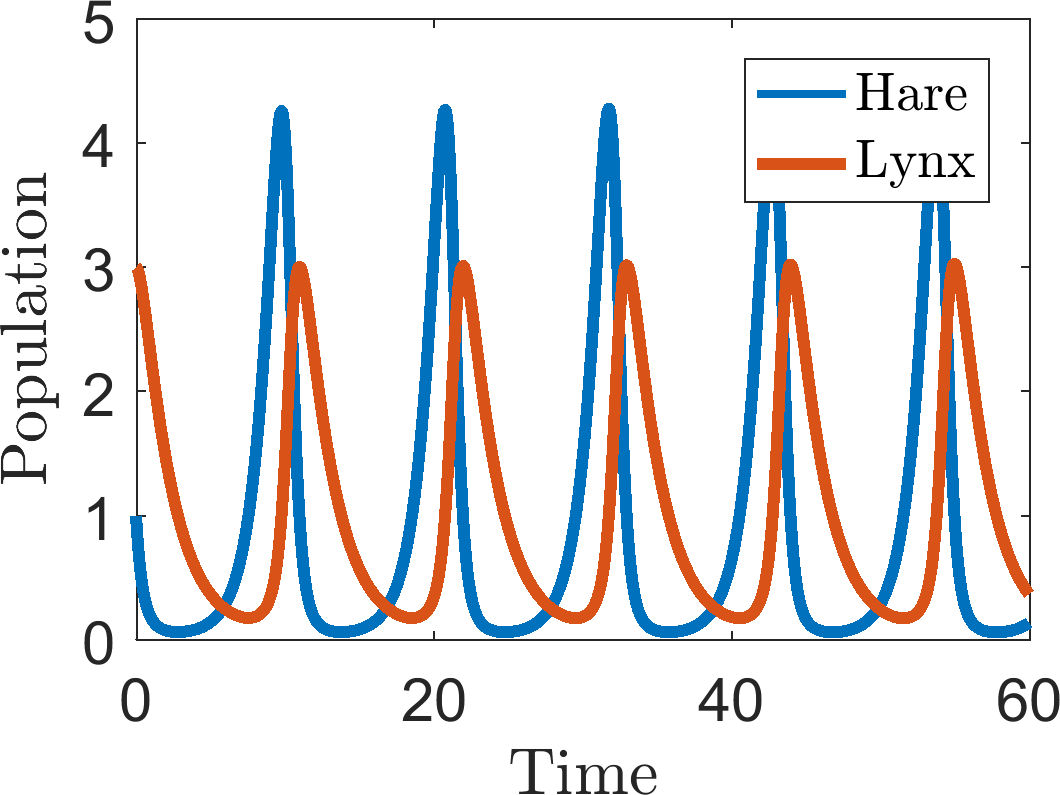
\includegraphics[height=\tttp]{../../Pictures/LV_time_sims.png}
\caption{Left: simulation of \eqns{LV1}{LV2}.\label{LV_time_sims}}
\end{figure}
\end{Answ}


\section{Bifurcations}
Consider the following set of equations which model the interactions of two populations $N_1$ and $N_2$:
\begin{align}
\dot{N}_1&=r_1N_1\l 1-\frac{N_1}{K_1+b_{12}N_2}\r,\\
\dot{N}_2&=r_2N_2\l 1-\frac{N_2}{K_1+b_{21}N_1}\r.
\end{align}
\begin{enumerate}
\item What dynamics are occurring between the species $N_1$ and $N_2$?

Hint 1: by the symmetry of $N_1$ and $N_2$ in the equations whatever $N_1$ is doing to $N_2$, $N_2$ is doing to $N_1$. This means that the dynamics could be mutual creation (mutualism) or mutual destruction (competition).

Hint 2: Compare the above equations to regular logistic curve $\dot{u}=ru(1-u/K)$. What happens if we increase or decrease $K$? Thus, what influence does increasing or decreasing $N_1$ have on $N_2$?

\item Use $N_1=K_1u_1$, $N_2=K_2u_2$, $\tau=r_1t$ to non-dimensionalise the equations. Define $\rho=r_2/r_1$, $\alpha_{12}=b_{12}k_2/k_1$ and $\alpha_{21}=b_{21}k_1/k_2$. Rewrite the system parameters in terms of $\alpha_{12}$, $\alpha_{21}$ and $\rho$.

\item Show that the system has four steady states:
\bb
(0,0), \quad (0,1), \quad (1,0), \quad (\bar{u}_1,\bar{u}_2), \quad
\ee
where
\bb
\bar{u}_1=\frac{1+\alpha_{12}}{1-\alpha_{12}\alpha_{21}},\quad\bar{u}_2=\frac{1+\alpha_{21}}{1-\alpha_{12}\alpha_{21}}.
\ee
What restrictions (if any) do we need to place of the steady states?
\item Determine the linear stability of the steady states. Taking care to note any bifurcation conditions and how they relate to the restrictions on the steady state existence.
\end{enumerate}
\begin{Answ}
\subsection{Answers}
\subsubsection{}
An increase in $N_1$ causes and increase in the steady state of $N_2$, thus, we have mutualism. Namely the population both cause each other to grow.
\subsubsection{}
The equations simplify to:
\begin{align}
\dot{u}_1&=u_1\l 1-\frac{u_1}{1+\alpha_{12}u_2}\r,\\
\dot{u}_2&=\rho u_2\l 1-\frac{u_2}{1+\alpha_{21}u_1}\r.
\end{align}
\subsubsection{}
Setting $\dot{u}_1=\dot{u}_2=0$ provides the given steady states. Note that we need $\alpha_{12}\alpha_{21}>1$ for $(\bar{u}_1,\bar{u}_2)$ to make sense as a positive steady state, since we are dealing with populations.
\subsubsection{}
The Jacobian is
\bb
J(u_1,u_2)=\left[ {\begin{array}{cc}
   1-\frac{2u_1}{1+\alpha_{12}\alpha_{21}u_2} & \frac{a u_1^2}{\l 1+\alpha_{12}\alpha_{21}u_2\r^2} \\
   \frac{\rho u_2^2}{\l 1+\alpha_{12}\alpha_{21}u_1\r^2} & \rho -\frac{2\rho u_2}{1+\alpha_{12}\alpha_{21}u_1} \\
  \end{array} } \right],
\ee
and so
\bb
J(0,0)=\left[ {\begin{array}{cc}
   1 & 0 \\
   0 & \rho \\
  \end{array} } \right],
\ee
meaning that $(0,0)$ is an unstable node.
\bb
J(0,1)=\left[ {\begin{array}{cc}
   1 & 0 \\
   a\rho & -\rho \\
  \end{array} } \right],
\ee
meaning that $(0,1)$ is a saddle.
\bb
J(1,0)=\left[ {\begin{array}{cc}
   -1 & a \\
   0 & \rho \\
  \end{array} } \right],
\ee
meaning that $(1,0)$ is a saddle.
\bb
J(\bar{u}_1,\bar{u}_2)=\left[ {\begin{array}{cc}
   -1 & \alpha_{12} \\
   \rho\alpha_{21} & -\rho \\
  \end{array} } \right].
\ee
Calculating the eigenvalues, $\lambda$, of $J(\bar{u}_1,\bar{u}_2)$ we find that
\bb
\lambda^2 +\underbrace{(1+\rho)}_{>0}\lambda+\underbrace{\rho(1-\alpha_{12}\alpha_{21})}_{>0}=0.
\ee
Since the coefficient of $\lambda$ and the constant term are positive (equally the trace and determinant of $J(\hat{u}_1,\hat{u}_2)$ are negative and positive, respectively), then $(\bar{u}_1,\bar{u}_2)$ is stable whenever it exists.
\end{Answ}

\section*{Exam revision}
\section{Predator competition}
One of the assumptions in the Lotka-Volterra equation is that the predation effect is proportional to both the predator and prey population. However, as the number of prey increases the  competition between predators will increase, thus, we consider the adapted equations
\begin{align}
\dot{u}=u-uv,\\
\dot{v}=b(uv-v)-bv^2.
\end{align}
\begin{enumerate}
\item What are the steady states of the system?
\item Characterise the stability of the valid steady states, noting any dependences on the parameter $b$.
\item How does predator competition change the outcome of the situation, compared to the basic Lotka-Volterra equation shown in question \ref{Lotka-Volterra equations}?
\end{enumerate}
\begin{Answ}
\subsection{Answer}
\subsubsection{}
The steady states are $(0,0)$, $(0,-1)$ and $(2,1)$.
\subsubsection{}
The Jacobian is
\bb
J(u,v)=\left[ {\begin{array}{cc}
   1-v & -u \\
   bv & b(u-1-2v) \\
  \end{array} } \right],
\ee
so, 
\bb
J(0,0)=\left[ {\begin{array}{cc}
   1 & 0 \\
   0 & -b \\
  \end{array} } \right],
\ee
meaning that (0,0) is a saddle point.
\bb
J(2,1)=\left[ {\begin{array}{cc}
   0 & -2 \\
   b & -b \\
  \end{array} } \right].
\ee
The eigenvalues satisfy
\bb
\lambda^2+b\lambda+2b=0,\quad\implies\lambda_\pm=\frac{-b\pm\sqrt{b(b-8)}}{2}.
\ee
For $0\leq b < 8$ $\lambda_\pm$ is complex and the real part is negative, so we have a stable spiral. For $b\geq 8$ $\lambda_-<\lambda_+<0$ and so we have a stable node.
\subsubsection{}
In the basic Lotka-Volterra case, all trajectories are closed, periodic orbits. In the case of predator competition the non-zero steady state is always stable.
\end{Answ}


\section{The Lorenz equations}
In 1963, Edward Lorenz developed a simplified mathematical model for atmospheric convection. The model is a system of three ordinary differential equations now known as the Lorenz equations:
\begin{align}
\dot{x}&=\sigma (y-x),\\
\dot{y}&=x(\rho -z)-y,\\
\dot{z}&=xy-\beta z.
\end{align}
The equations relate the properties of a two-dimensional fluid layer uniformly warmed from below and cooled from above. In particular, the equations describe the rate of change of three quantities with respect to time: $x$ is proportional to the rate of convection; $y$ is proportional to the horizontal temperature variation; $z$ is proportional to the vertical temperature variation. The constants $\sigma$, $\rho$, and $\beta$ are system parameters proportional to the Prandtl number, Rayleigh number, and certain physical dimensions of the layer itself.

For simplicity, let $\sigma=\beta=1$.
\begin{enumerate}
\item What are the steady states, noting dependencies of $\rho$?
\item Characterise the stability of the  zero steady state only, noting dependencies of $\rho$. Note that you will have to find the eigenvalues of a $3\times 3$ matrix. Substituting in the values of the steady state will help you. The non-zero steady states are always either stable nodes or stable spirals when they exist.
\item Simulations for $\rho>1$ and $\rho<1$ are illustrated in \fig{Lorenz_stable}. Do these accord with your findings?
\end{enumerate}

EXTENSION 1: If you are brave enough calculate the eigenvalues corresponding to the non-zero steady states and show that they always have negative real part when $\rho>1$, but they may be complex.

EXTENSION 2: If you are even braver rerun the analysis with variables $\sigma=10$, $\rho=28$ and $\beta=3$. This causes the system to act chaotically. Categorise the steady states in this case. What happens? An image of the chaotic trajectory can be seen in \fig{Lorenz_chaotic}.
\begin{figure}[h!!!tb]
\centering
\subfigure[\label{rho_0.5}$\rho=0.5$]{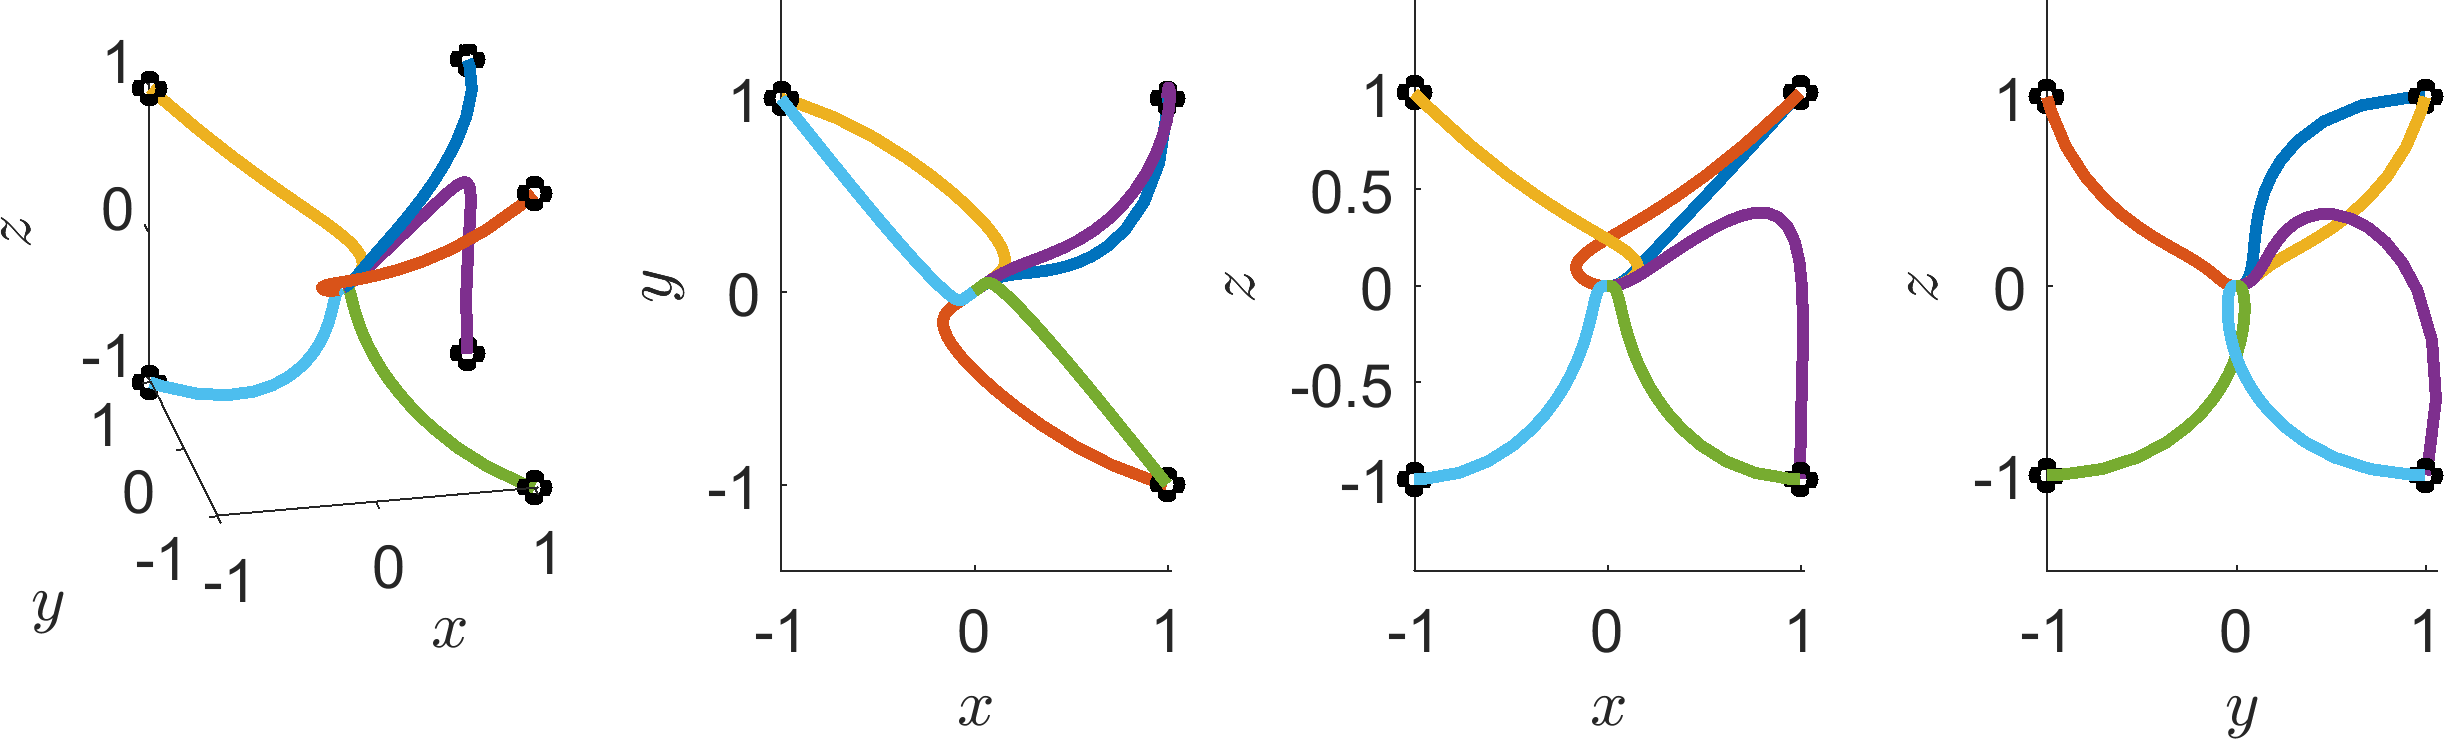
\includegraphics[width=\tp]{../../Pictures/Lorenz_sims_rho_5.png}}
\subfigure[\label{rho_2}$\rho=2$]{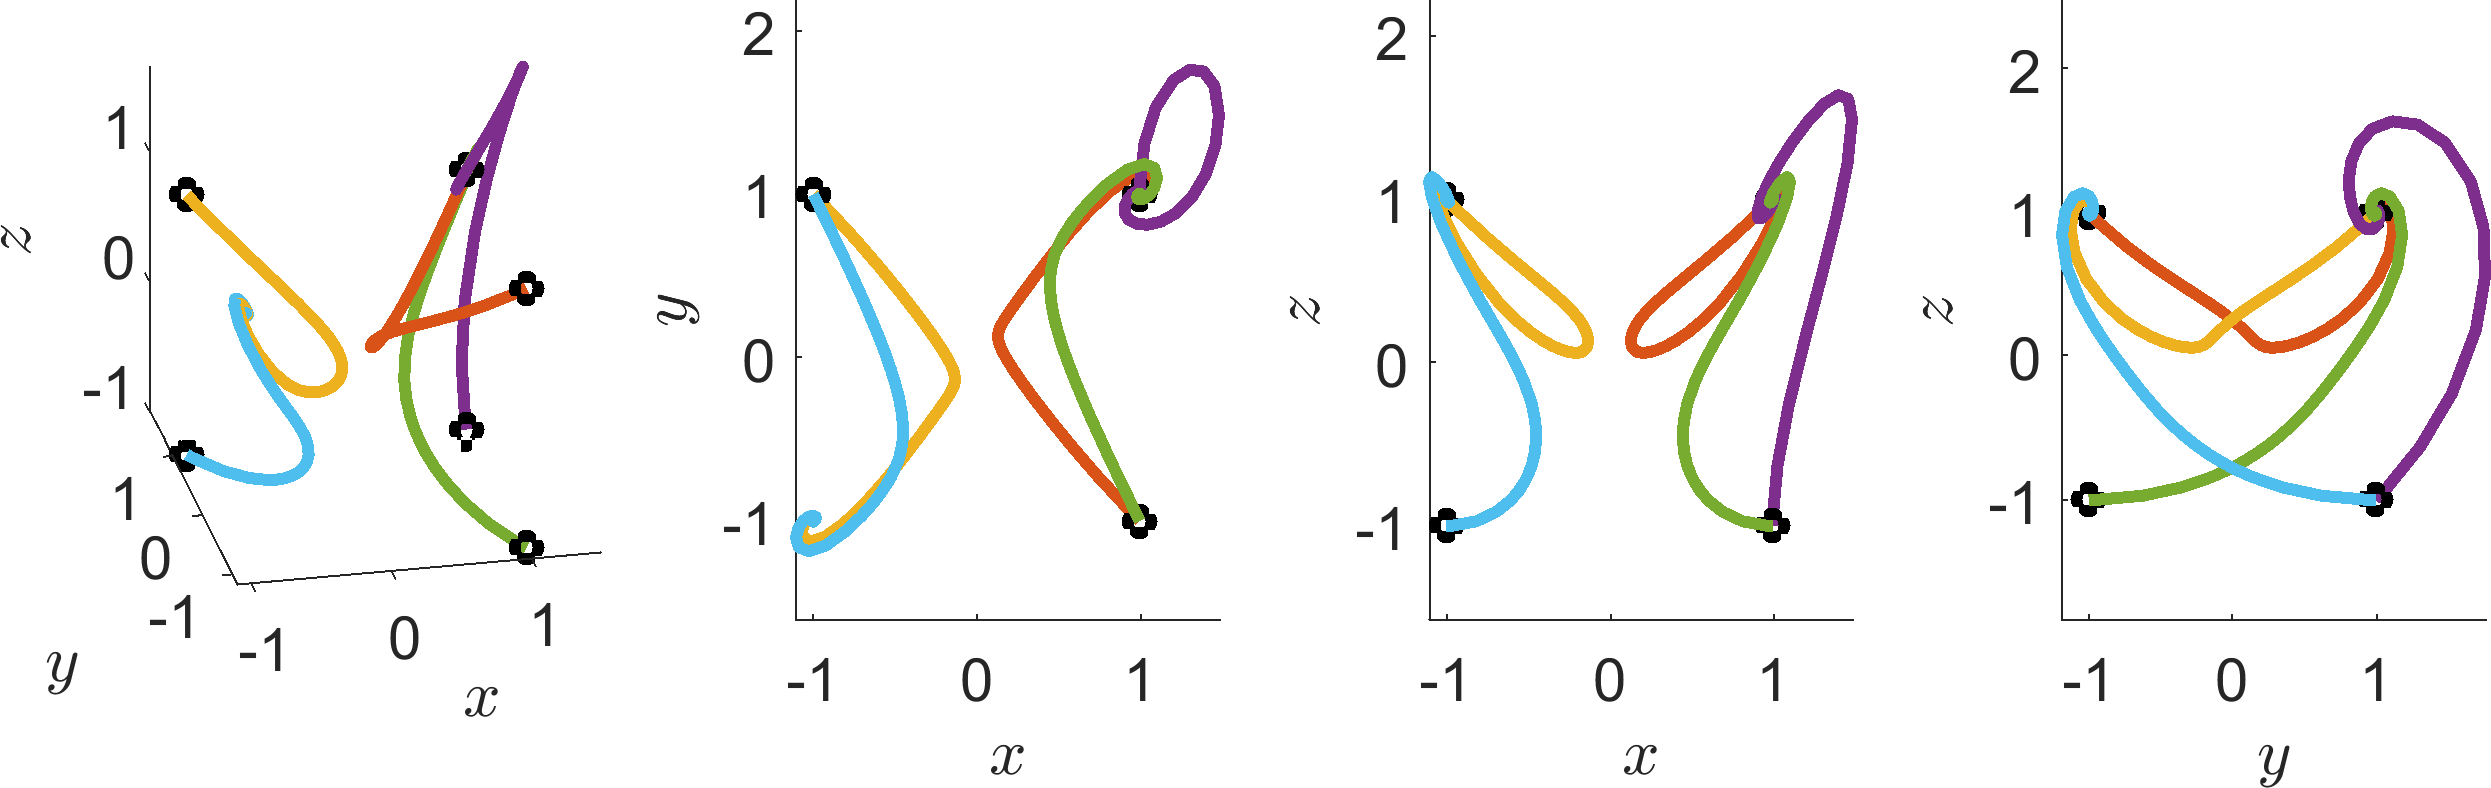
\includegraphics[width=\tp]{../../Pictures/Lorenz_sims_rho_20.png}}
\caption{\label{Lorenz_stable} Simulating the Lorenz equations with $\sigma=1$, $\beta=1$ and $\rho$ given beneath each figure, for a variety of initial conditions. The black circles indicate the initial conditions. On the left is the full, three-dimensional realisation, whilst the rest of the plots in the row are the $(x,y)$, $(x,z)$ and $(y,z)$ projections.}
\end{figure}


\begin{figure}[h!!!tb]
\centering
\subfigure[]{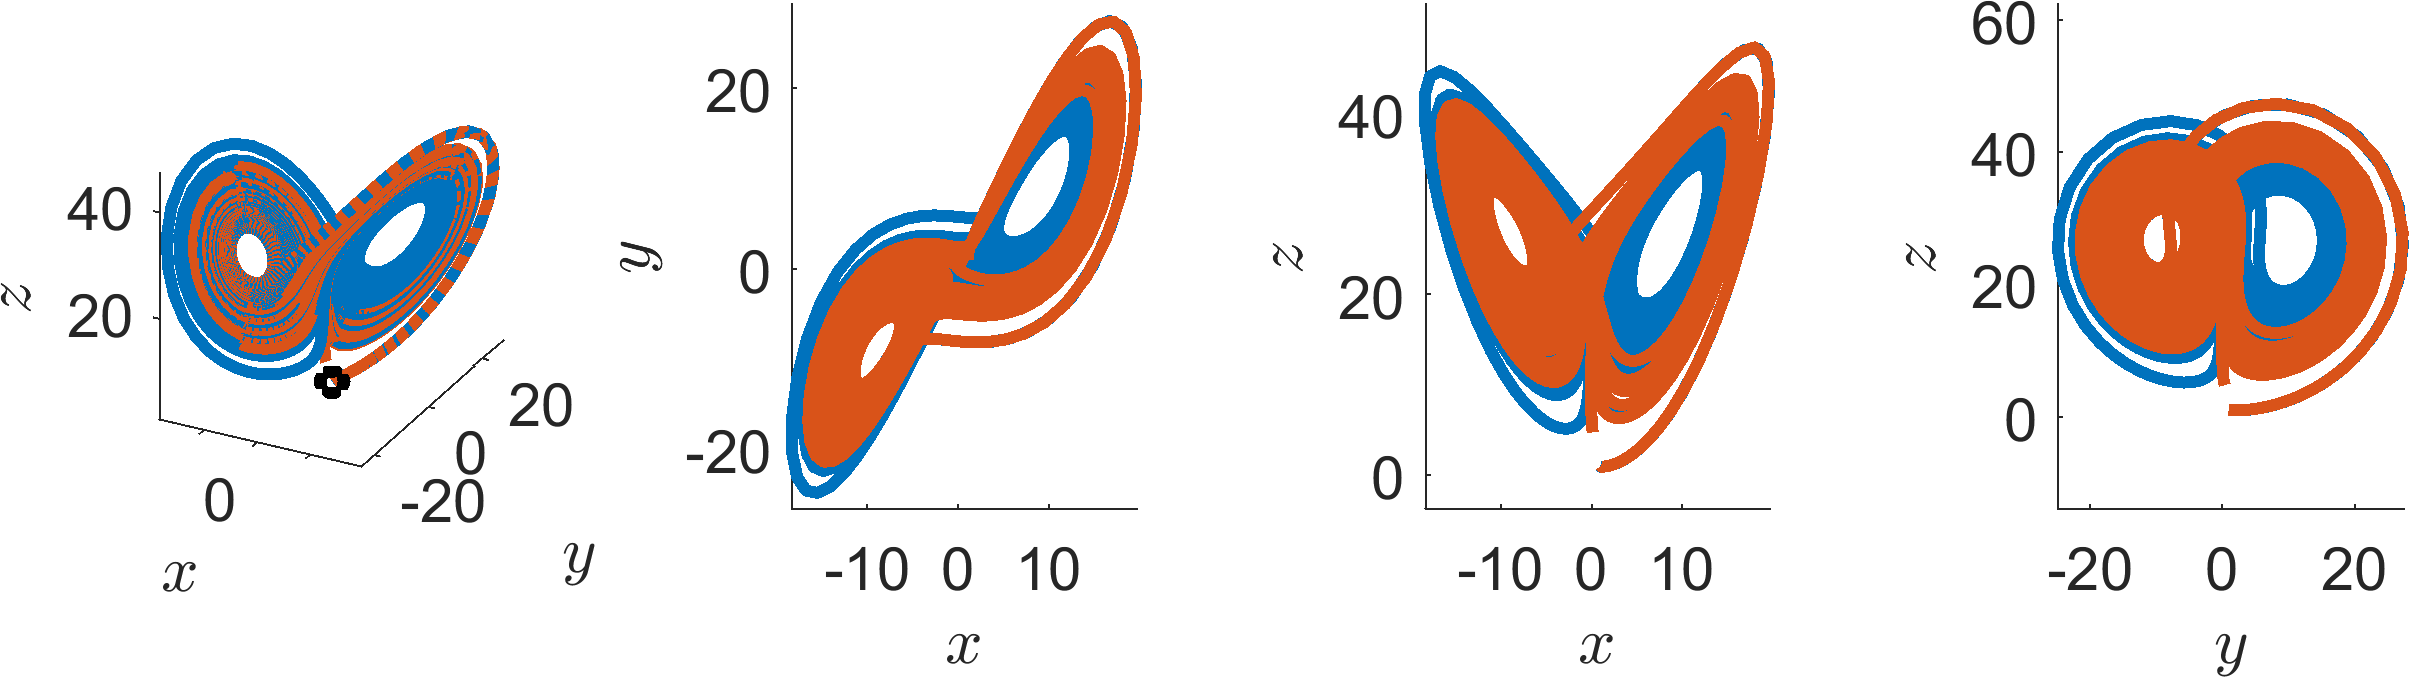
\includegraphics[width=\tp]{../../Pictures/Lorenz_sims_rho_280.png}}
\subfigure[]{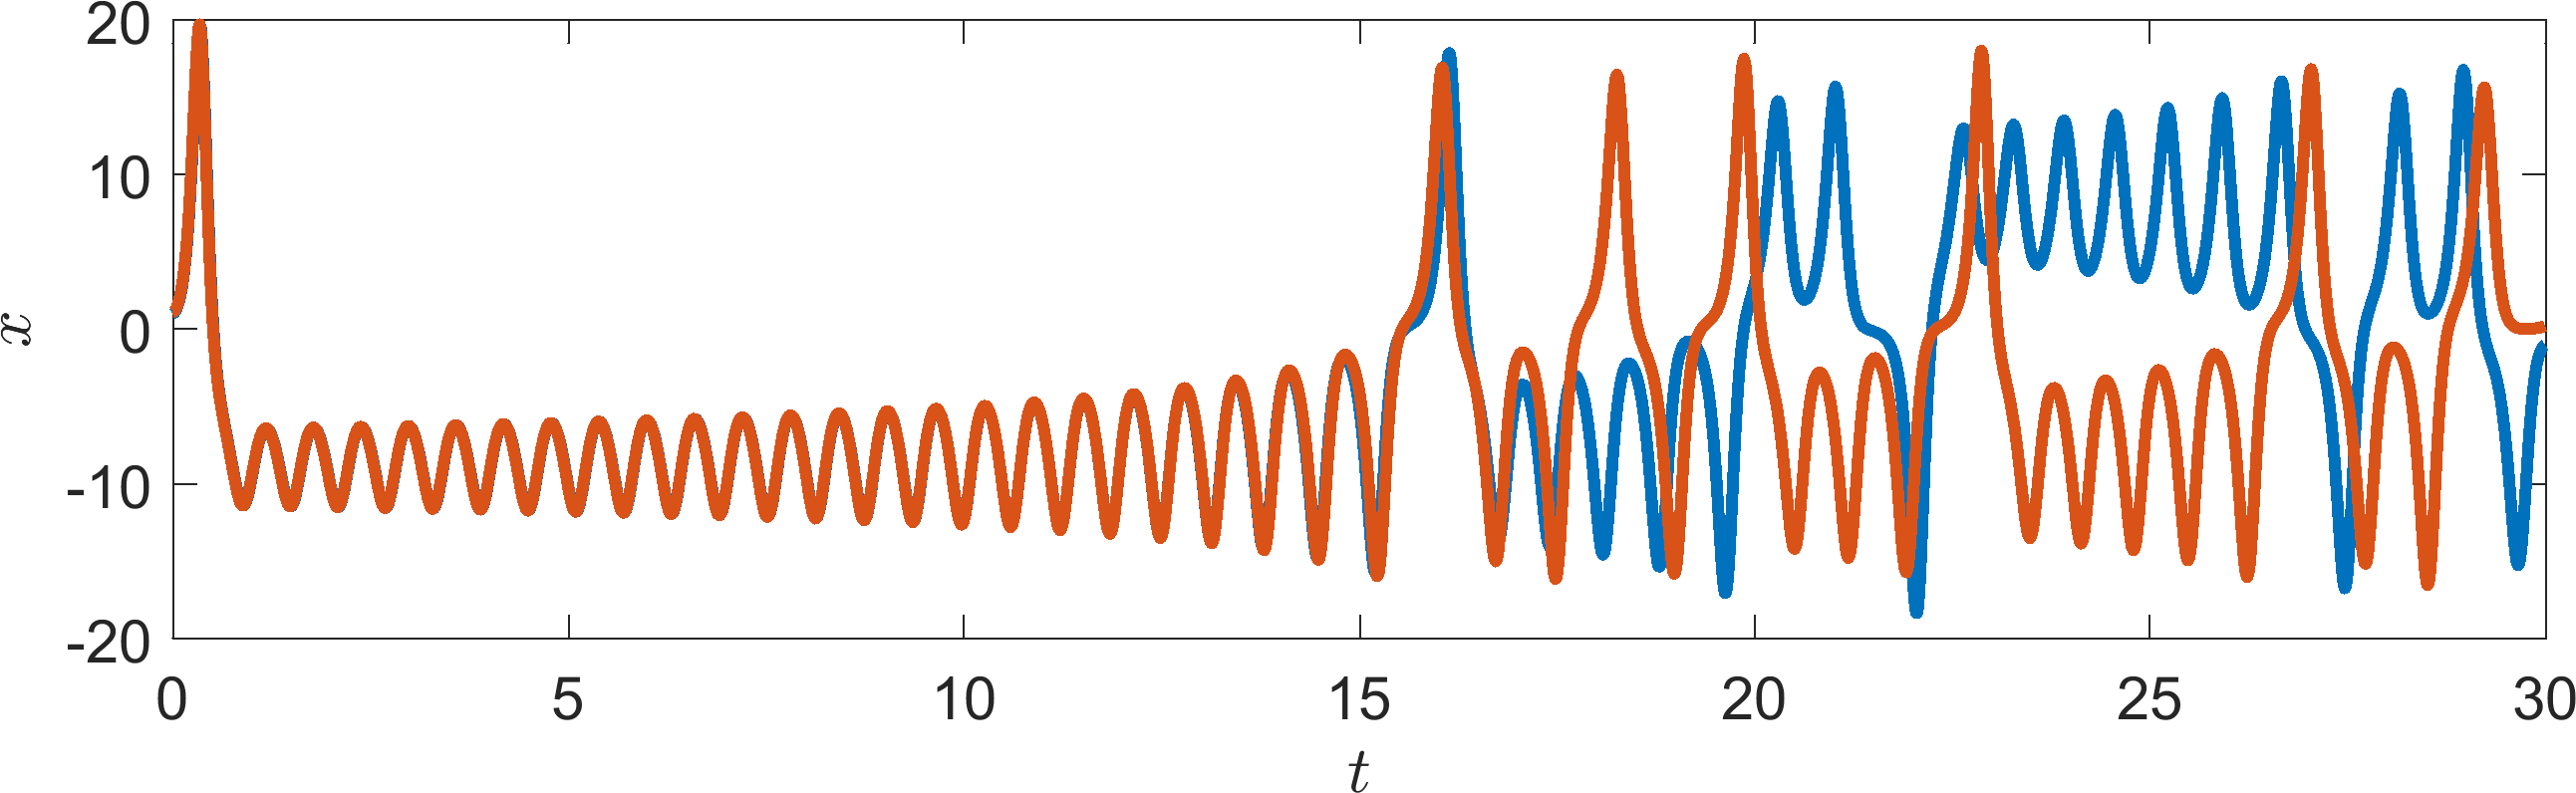
\includegraphics[width=\tp]{../../Pictures/Lorenz_chaos.png}}
\caption{\label{Lorenz_chaotic} Simulating the Lorenz equations with $\sigma=10$, $\beta=3$ and $\rho=28$ for two initial conditions that start very close together. Top: the black circles indicate the initial conditions. On the left is the full, three-dimensional realisation, whilst the rest of the plots in the row are the $(x,y)$, $(x,z)$ and $(y,z)$ projections. Bottom: time series of $x$, where we observe the two trajectories diverging.}
\end{figure}
\begin{Answ}
\subsection{Answers}
\subsubsection{}
There are three steady states:
\bb
(0,0,0), \quad(\pm\sqrt{\rho-1},\pm\sqrt{\rho-1},\rho-1).
\ee
and we note that we need $\rho>1$ for the non-zero states to exist.
\subsubsection{}
The Jacobian is
\bb
J(x,y,z)=\left[ {\begin{array}{ccc}
   -1 & 1 & 0 \\
   r-z & -1 & -x \\
   y  & x & -1 \\
  \end{array} } \right].
\ee
\bb
J(0,0,0)=\left[ {\begin{array}{ccc}
   -1 & 1 & 0 \\
   \rho & -1 & 0 \\
   0 & 0 & -1 \\
  \end{array} } \right],
\ee
thus, the eigenvalues satisfy the equation
\bb
(-1-\lambda)((-1-\lambda)^2-\rho)=0,\quad \implies\lambda_{-1}=-1,\quad\lambda_{\pm}=-1\pm\sqrt{\rho}.
\ee
Hence, $(0,0,0)$ is stable if $0<\rho<1$ and unstable if $\rho>1$.
\subsubsection{}
The simulations in \fig{Lorenz_stable} show that when $0<\rho<1$ the steady state always tends to the origin. However, for $\rho>1$, the trajectory tends to one of the non-zero steady states depending on the initial condition.



\subsubsection{EXTENSION 1}
The stability of the $(\pm\sqrt{\rho-1},\pm\sqrt{\rho-1},\rho-1)$ states are both the same. Here, we will illustrate how to extract the eigenvalues of $(\sqrt{\rho-1},\sqrt{\rho-1},\rho-1)$, the negative case is similar.
\bb
J(\sqrt{\rho-1},\sqrt{\rho-1},\rho-1)=\left[ {\begin{array}{ccc}
   -1 & 1 & 0 \\
   1 & -1 & -\sqrt{\rho-1} \\
   \sqrt{\rho-1}  & \sqrt{\rho-1} & -1 \\
  \end{array} } \right],
\ee
thus, the eigenvalues satisfy the equation
\begin{align}
0&=(-1-\lambda)((-1-\lambda)^2+(\rho-1))-((-1-\lambda)+(\rho-1)),\\
&=\lambda^3+3\lambda^2+(1+\rho)\lambda+2(\rho-1),\\
&=(\lambda+2)(\lambda^2+\lambda+\rho-1).\\
\end{align}
Hence,
\bb
\lambda_{-2}=-2,\quad\lambda_{\pm}=\frac{-1\pm\sqrt{5-4\rho}}{2},
\ee
and all eigenvalues have negative real part whenever $\rho>1$.

\subsubsection{EXTENSION 2}
In the case that  $\sigma=10$, $\rho=28$ and $\beta=3$ the eigenvalues relating to $(0,0,0)$ are
\bb
\lambda_1\approx-22.8,\quad\lambda_2\approx 11.8\quad\lambda_3=-3.
\ee
So the state is unstable. The non-zero steady states are $(\pm9,\pm9,27)$, the accompanying eigenvalues are
\bb
\lambda_1\approx-14.1,\quad\lambda_2\approx 0.04+10.7I\quad\lambda_3=0.04-10.7I.
\ee
Thus, these states are also unstable. Normally, when all steady steady states are unstable we would expect the trajectory to tend to infinity along one of the coordinates, creating a singularity. However, the trajectories in these simulations are always bounded, thus, they cannot escape to infinity. Equally, they can not oscillate around one of the critical point because otherwise it would be a centre and not unstable. Thus, something more complicated must be occurring. Namely, chaos!
\end{Answ}
%
%\section{Michaelis-Menten Enzyme dynamics}
%Enzymes are biological molecules (typically proteins) that significantly speed up the rate of virtually all of the chemical reactions that take place within cells. They are vital for life and serve a wide range of important functions in the body, such as aiding in digestion and metabolism.
%\begin{figure}[h!!!tb]
%\centering
%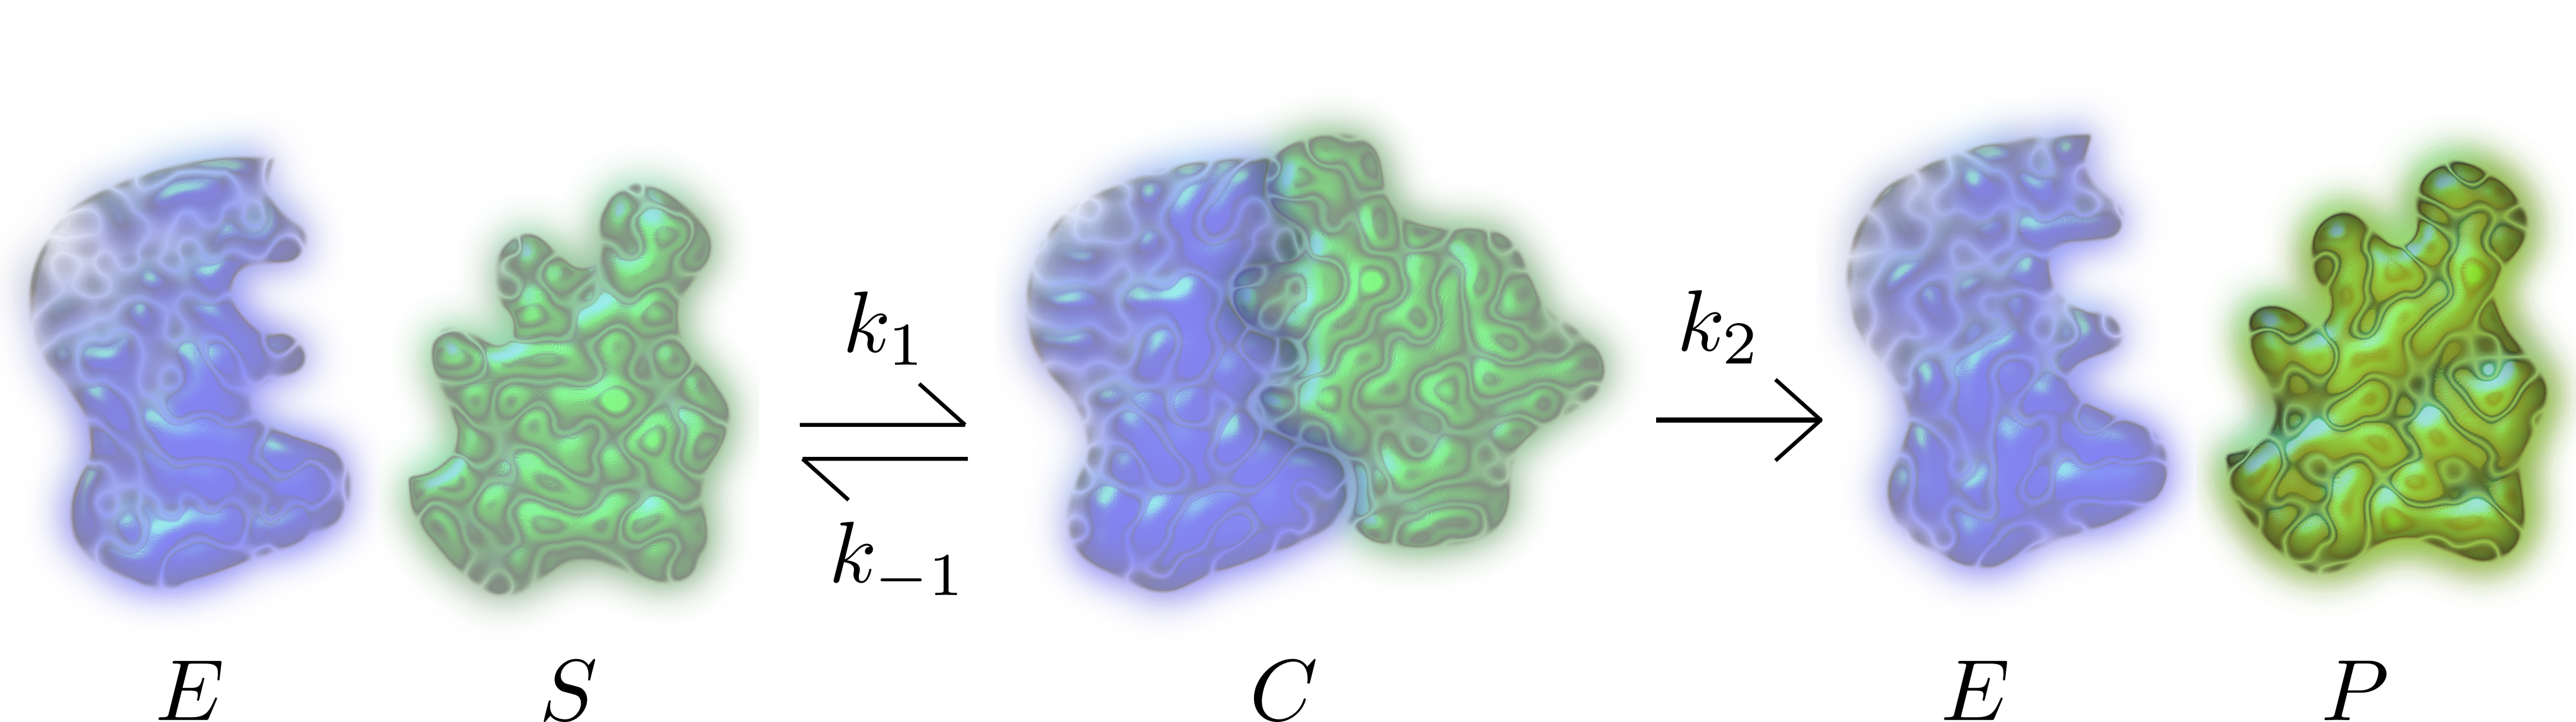
\includegraphics[width=\textwidth]{../../Pictures/Michaelis-Menten_schematic.png}
%\caption{\label{Michaelis-Menten_schematic} Schematic diagram of the Michaelis-Menten enzyme-substrate reaction.}
%\end{figure}
%
%In 1913 Leonor Michaelis and Maud Menten proposed a mathematical model of how enzymes work. The process involves an enzyme, $E$, binding to a substrate, $S$, to form a complex, $C$, which in turn releases a product, $P$, regenerating the original enzyme. This may be represented schematically as
%\bb
%E+S\mathrel{\mathop{\rightleftarrows}^{k_1}_{k_{-1}}}C\stackrel{k_2}{\rightarrow}E+P.
%\ee
%\begin{enumerate}
%\item Use the Law of Mass Action to right down the ODE formulation of the dynamics. The initial conditions are
%\bb 
%S(0) = S_0,\quad E(0) = E_0,\quad C(0) = 0,\quad P(0) = 0.
%\ee
%\item Show $E+C=$constant$=E_0$.
%\item Why can we ignore the equations for $\dot{P}$ and $\dot{E}$? Specifically, show that we only need to consider the equations
%\begin{align}
%\dot{S}&=-k_1(E_0-C)S + k_{-1}C,\\
%\dot{C}&=k_1(E_0-C)S -( k_{-1}+k_2)C.
%\end{align}
%\item Use the following scales to non-dimensionalise the equations
%\bb
%t=\frac{\tau}{k_1E_0}\quad S=u S_0\quad C=v E_0,
%\ee
%to produce the following system
%\begin{align}
%\frac{\rd u}{\rd \tau}&=-u+(u+K-\lambda)v,\label{u}\\
%\epsilon\frac{\rd v}{\rd \tau}&=u-(u+K)v\label{v}.
%\end{align}
%What are $\epsilon$, $\lambda$ and $K$? Show that $\epsilon$, $\lambda$ and $K$ are non-dimensional.
%\item What are the initial conditions?
%\item \label{Inner}Suppose $E_0\ll S_0$ (what does this mean?) and substitute the time scale $\sigma=\tau/\epsilon$ into \eqns{u}{v}. You should be able to show that the solution of the system is
%\begin{align}
%u(\sigma)&=1,\nonumber\\
%v(\sigma)&= \frac{1}{1+K}\l 1-\exp(-(1+K)\sigma)\r.
%\end{align}
%Hint: $E_0\ll S_0\implies \epsilon\ll 1$, thus, once the equations have been multiplied take the limit of $\epsilon\rightarrow 0$ in the $\rd u/ \rd \sigma$ equation. Solve this and substitute the solution for $u$ in the $\rd v/ \rd \sigma$ equation.
%
%\item Return to \eqns{u}{v} and let $\epsilon\rightarrow0$. Show that we can write $v$ as a function of $u$, which simplifies the $\rd u/\rd \tau$ equation to
%\bb
%\frac{\rd u}{\rd \tau}=-u+(u+K-\lambda)\frac{u}{(u+K)}, \quad u(0)=1.
%\ee \label{Outer}
%\end{enumerate}
%In questions \ref{Inner}-\ref{Outer} you have done a multiple scales simplification of the Michaelis-Menton problem. Namely, the whole equation is hard to solve. However, we can solve for what the equation looks like for small time, $\sigma$ (question \ref{Inner}) and we can solve for what the equations looks like for large time, question (\ref{Outer}). In the computation question, which is next, we check these approximations.
%
%\subsection{Answers}
%\subsubsection{}
%\begin{align}
%\dot{E}&=-k_1ES+\l k_{-1}+k_2\r C,\nonumber\\
%\dot{S}&=-k_1ES+k_{-1} C,\nonumber\\
%\dot{C}&=k_1ES-\l k_{-1}+k_2\r C,\nonumber\\
%\dot{P}&=k_2C\nonumber.
%\end{align}
%\subsubsection{}
%\bb
%\rd\l E+C\r/\rd t=0\implies E+C=\textrm{ constant }=E_0,
%\ee
%using the initial conditions.
%\subsubsection{}
%$\dot{P}$ depends on $C$, but none of the other equations depend on $P$, thus, $\dot{P}$ decouples from the system, in that once we solved the rest of the system we can produce $P$ through integration $C$. This leaves equations for $E$, $S$ and $C$. Using $E+C=E_0$ we can eliminate $E$ as well, leaving just equations for $S$ and $C$. Substituting in $E=E_0-C$ we generate
%\begin{align}
%\dot{S}&=-k_1(E_0-C)S + k_{-1}C,\\
%\dot{C}&=k_1(E_0-C)S -( k_{-1}+k_2)C.
%\end{align}
%\subsubsection{}
%We should find that
%\begin{align}
%\epsilon&=\frac{E_0}{S_0},\nonumber\\
%\lambda&=\frac{k_2}{k_1S_0},\nonumber\\
%K&=\frac{k_{-1}+k_2}{k_1S_0}\nonumber.
%\end{align}
%The units are:\\
%dim($\epsilon$)=density/density=1,\\
%dim($\lambda$)=$\frac{\textrm{1/time}}{1/(\textrm{density}\times \textrm{time}) \times \textrm{density}}=1=$dim($K$).
%\subsubsection{}
%The initial conditions are $u(0)=S_0/S_0=1$ and $v(0)=0/E_0=0$.
%
%\subsubsection{}
%$E_0\ll S_0$ means that there is very little enzyme compared to substrate.
%On substituting $\sigma=\tau/\epsilon$ into \eqns{u}{v} we have 
%\begin{align}
%\frac{\rd u}{\rd \sigma}&=\epsilon\l-u+(u+K-\lambda)v\r\approx 0,\quad u(0)=1\label{u_inner}\\
%\frac{\rd v}{\rd \sigma}&=u-(u+K)v\quad v(0)=0.\label{v_inner}
%\end{align}
%Solve \eqn{u_inner} provides $u=1$, which is substituted into \eqn{v_inner} to produce
%\bb
%\frac{\rd v}{\rd \sigma}=1-(1+K)v\quad v(0)=0.
%\ee
%Solving this equations gives the final answer
%\bb
%v(\sigma)= \frac{1}{1+K}\l 1-\exp(-(1+K)\sigma)\r.
%\ee
%\subsubsection{}
%Setting $\epsilon=0$ in \eqn{v} gives
%\bb
%0=u-(u+K)v\implies v=u/(u+K),
%\ee
%which can be substituted into \eqn{u} to produce
%\bb
%\frac{\rd u}{\rd \tau}=-u+(u+K-\lambda)u/(u+K),\quad u(0)=1.\ee
%
%\section{Computer simulation}
%Let $K=2$, $\lambda=1$ and $\epsilon=0.001$. Simulate
%\begin{align}
%\frac{\rd u}{\rd \tau}&=-u+(u+K-\lambda)v, \quad u(0)=1\\
%\epsilon\frac{\rd v}{\rd \tau}&=u-(u+K)v \quad v(0)=0.
%\end{align}
%and 
%\bb
%\frac{\rd u}{\rd \tau}=-u+(u+K-\lambda)u/(u+K),\quad u(0)=1.
%\ee
%with $v=u/(u+K)$ over the time $t\in[0,20]$. How well do these curves approximate each other?
%
%\subsection{Answer}
%The simulations are shown below.
%\begin{figure}[h!!!tb]
%\centering
%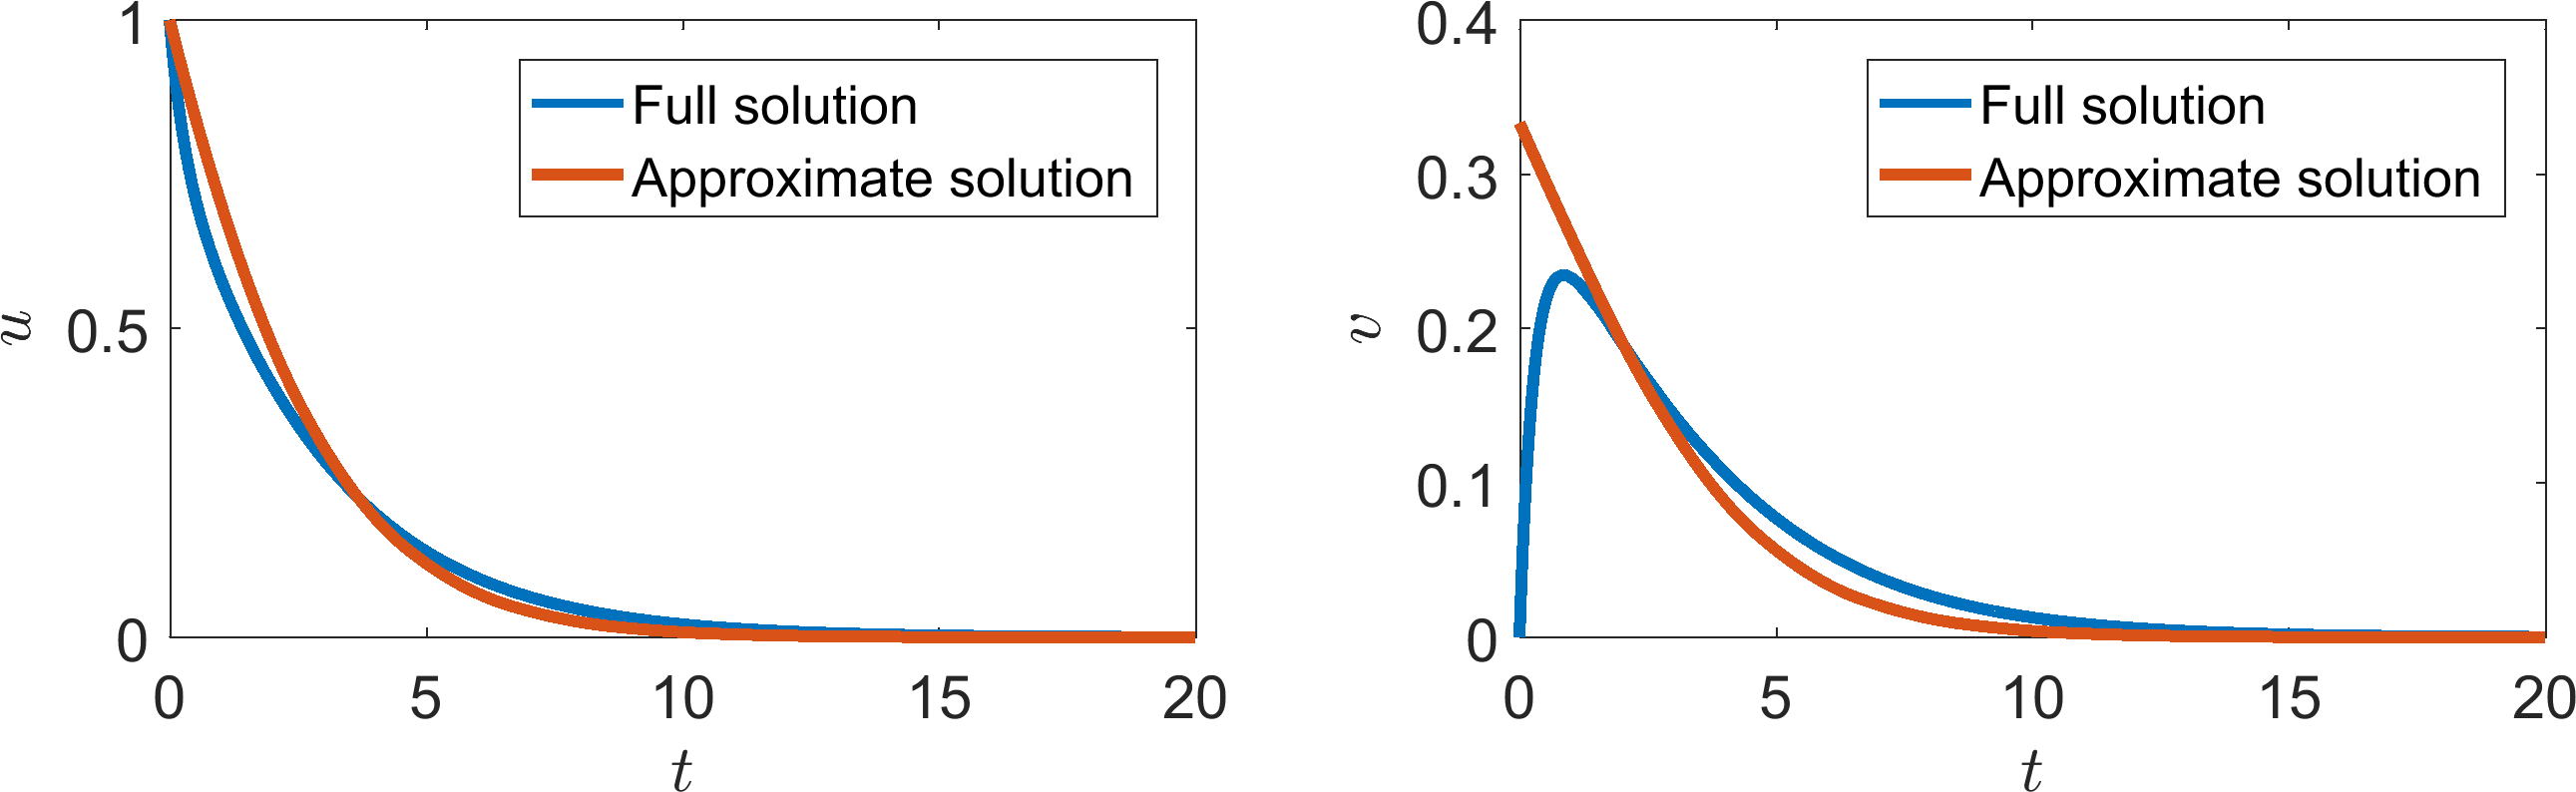
\includegraphics[width=\textwidth]{../../Pictures/Michaelis-Menten_approximation.png}
%\caption{\label{Michaelis-Menten} Full and approximate solutions to the Michaelis-Menten problem.}
%\end{figure}
%
%
%
%\section{Spruce budworm}
%\begin{figure}[h!!!tb]
%\centering
%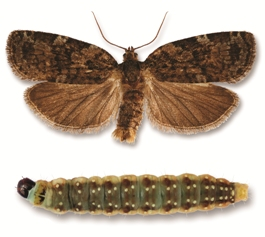
\includegraphics[width=\ttp]{../../Pictures/Spruce_budworm.jpg}
%\caption{\label{Spruce_budworm} Spruce budworm in moth and larval stages.}
%\end{figure}
%Spruce budworm \see{Spruce_budworm} are preyed upon by spiders, miscellaneous insects, and birds. A model for their population size, $N$ is given by
%\bb
%\dot{N}=RN\l 1-\frac{N}{K}\r-\frac{BN^2}{A^2+N^2}.
%\ee
%\begin{enumerate}
%\item What does each term in the equation mean?
%\item Describe, with a sketch, three properties of the predation term
%\bb
%\frac{BN^2}{A^2+N^2}.
%\ee
%Hint: consider low, medium and high values of $N$.
%\item Non-dimensionalise the equation to give the form
%\bb
%\frac{\rd u}{\rd \tau}=ru\l 1-\frac{u}{k}\r-\frac{u^2}{1+u^2}.
%\ee
%What are the scales of the population and time in terms of $A$, $B$, $K$ and $R$? What are the parameters $r$, $k$ in terms of $A$, $B$, $K$ and $R$?
%\item Show the population and time scales have the right dimension. Show that $r$ and $k$ are dimensionless.
%\end{enumerate}
%
%
%\subsection{Answers}
%\subsubsection{}
%\bb
%\underbrace{\dot{N}}_{\textrm{Population evolution.}}=\underbrace{RN\l 1-\frac{N}{K}\r}_{\textrm{Logistic growth, \ie linear growth with competition.}}-\underbrace{\frac{BN^2}{A^2+N^2}}_{\textrm{Predation effects.}}.
%\ee
%\subsubsection{}
%For low populations there is little predation. As the population grows, so does the predation. The predation saturates at large population.
%\subsubsection{}\label{Scales}
%\bb
%[N]=A,\quad [t]=\frac{A}{B},\quad r=\frac{RA}{B},\quad k=\frac{K}{A}.
%\ee
%\subsubsection{}
%$A$ has units of density, $B$ has units of density/time, $R$ has units of 1/time and $K$ has units of density.
%
%Substituting these into the scales in \sect{Scales} we find that $[N]$ and $[t]$ has units of density and time, respectively, whilst $r$ and $k$ are dimensionless.
%
%\section{Spruce budworm population stability}
%You can find more about the spruce budworm population equation and an online applet that allows you to simulate the system quickly and easily at the following website:
%\bb
%http://mathinsight.org/spruce\_budworm\_outbreak\_model
%\ee
%
%The above website may aid in the following questions as we are going to consider the steady states of
%\bb
%\frac{\rd u}{\rd \tau}=ru\l 1-\frac{u}{k}\r-\frac{u^2}{1+u^2}=f(u).\label{Spruce}
%\ee
%We could solve $f(u)=0$, however, this leads to a cubic in $u$. This can be solved, but it is not very fun. Instead, we are going to consider sketches of the system. 
%
%We could sketch $f(u)$, directly, and draw arrows on the diagram, such that $u$ is increasing if $f(u)>0$ and $u$ is decreasing if $f(u)<0$. This will immediately tell us how many stationary states there are and inform us of their stability. We will do this towards the end of this question, however, going straight into the full sketch may cause us to miss certain cases, as we have two parameters, $r$ and $K$, to worry about. However, if you feel confident shoot straight to question \ref{sketch_f}.
%
%Critically, the following questions only deal with sketches. Thus, you do not have to be exactly accurate in your plotted values. We are just need to provide the general shape of the curve. This means little, if any, calculation should be required. Namely, an exact analytical result is not required, only approximate sketches backed up by logical thought.
%
%\begin{enumerate}
%\item By inspection $u_0=0$ is always a steady state of $f(u)$ (make sure you understand why). Instead of considering $f(u)$ let us consider the two functions
%\bb
%f_1(u)=r\l 1-\frac{u}{k}\r,\quad f_2(u)=\frac{u}{1+u^2}.
%\ee
%Sketch $f_2$ on three different axes. Fix the value of $r/k$ to be greater than zero (say $r/k=0.05$), but allow $r$ to vary (with $k$ being defined by, say, $k=0.05/r$). Sketch on these three different plots $f_1$ for different values of $r$, namely consider $r$ small, medium and large\footnote{Note that small, medium and large values are ill-defined. Specifically, when saying such terms you should always specify compared to what. Namely, small, or large, compared to what value? Thus, if you are plotting these accurately consider $r\in [0.4,0.6]$.}
%
%
%
%\item Draw on your above diagrams regions where $f_1>f_2$ and regions where $f_2>f_1$.
%
%\item Noting that a steady state, $u'$, satisfies
%\bb
%f(u')=0=u'(f_1(u')-f_2(u')),
%\ee
%use your sketches of $f_1$ and $f_2$ to plot three situations of $f(u)$\label{sketch_f}.
%
%\item You should be able to show that (depending on the value of the parameters) there can be as few as two steady states and as many as 4 steady states. Name the four steady states $0=u_0<u_-<u_s<u_+$, in the obvious way. Specify on your diagrams these four steady states.  The middling value of $r$ sketch is given in \fig{r_medium}.
%\begin{figure}[h!!!tb]
%\centering
%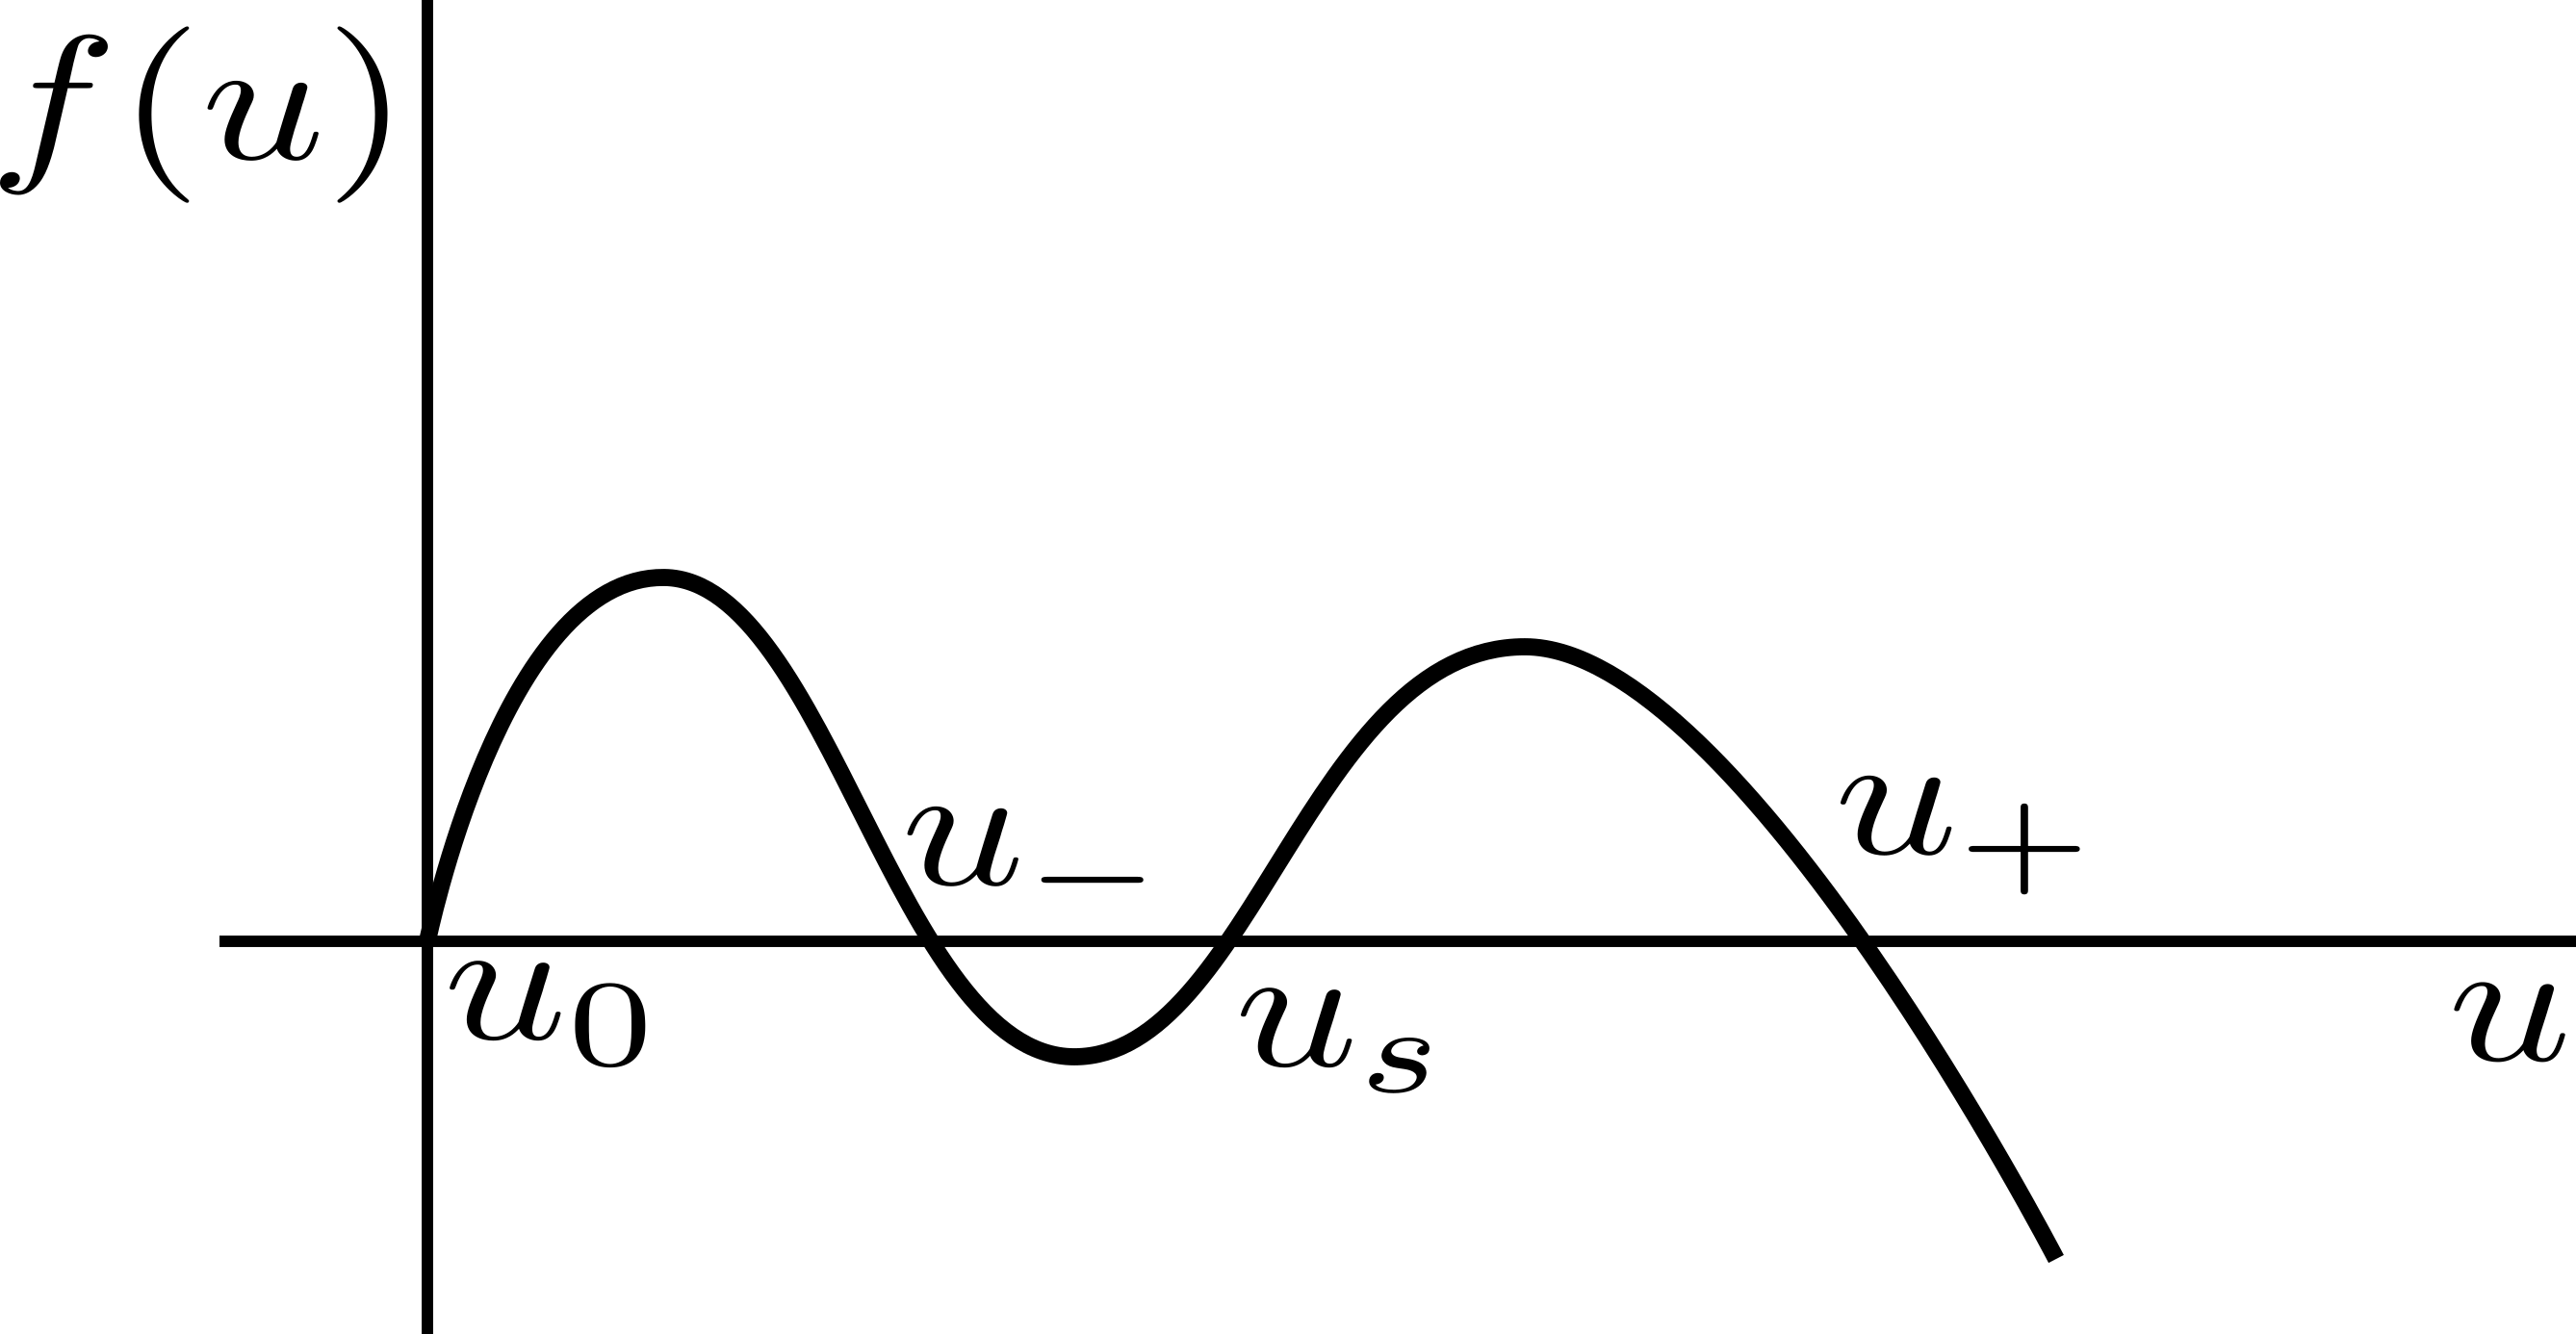
\includegraphics[width=\ttp]{../../Pictures/Spruce_budworm_r_medium.png}
%\caption{\label{r_medium} Plots of $f$ for a middling value of $r$.}
%\end{figure}
%
%\item Use each sketch of $f(u)$ to state the stability of each steady state, $u_0$, $u_-$, $u_s$ and $u_+$ (when they exist).
%
%
%\item Does the system exhibit hysteresis? To solve this follow these steps:
%\begin{enumerate}
%\item start with a low value of $r$, such that only $u_0$ and $u_-$  exist. Suppose to start with a small initial condition, where do you evolve to?
%\item increase $r$ until $u_0$, $u_-$, $u_s$, $u_+$ all exist, what happens to the point you evolve to?\label{1}
%\item increase $r$ further until only $u_0$ $u_+$ exist, what happens to the point you evolve to?
%\item decrease $r$ until $u_0$, $u_-$, $u_s$, $u_+$ all exist, what happens to the point you evolve to?\label{2}
%\item is the point you evolve to in step \ref{1} the same as the point you evolve to in step \ref{2}? Use this to answer the original question.
%\end{enumerate} 
%
%\end{enumerate}
%\subsection{Answer}
%\subsubsection{}
%$u=0$ is a solution of $f(u)=0$, thus, it is always a steady state. See \fig{f1_f2} for the sketches.
%\begin{figure}[h!!!tb]
%\centering
%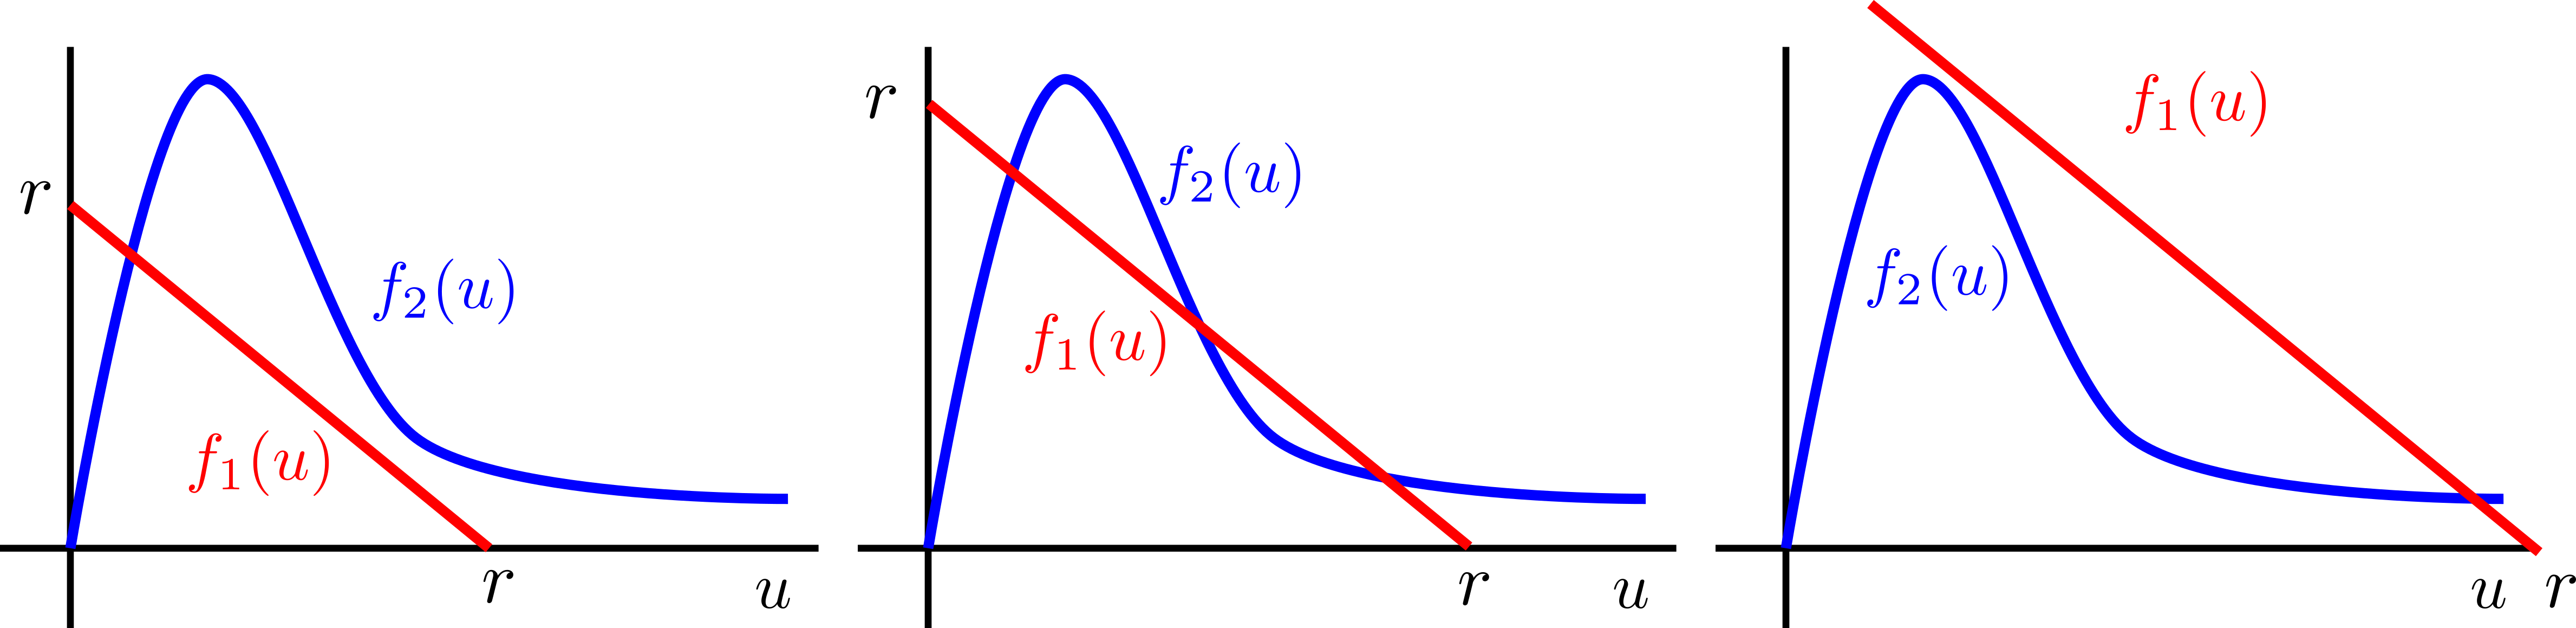
\includegraphics[width=\textwidth]{../../Pictures/f1_f2.png}
%\caption{\label{f1_f2} Plots of $f_1$ and $f_2$, for varying $r$ and fixed $r/k$. $r$ increases left to right.}
%\end{figure}
%\subsubsection{}
%See \fig{f1_f2_positivity} for the sketches.
%\begin{figure}[h!!!tb]
%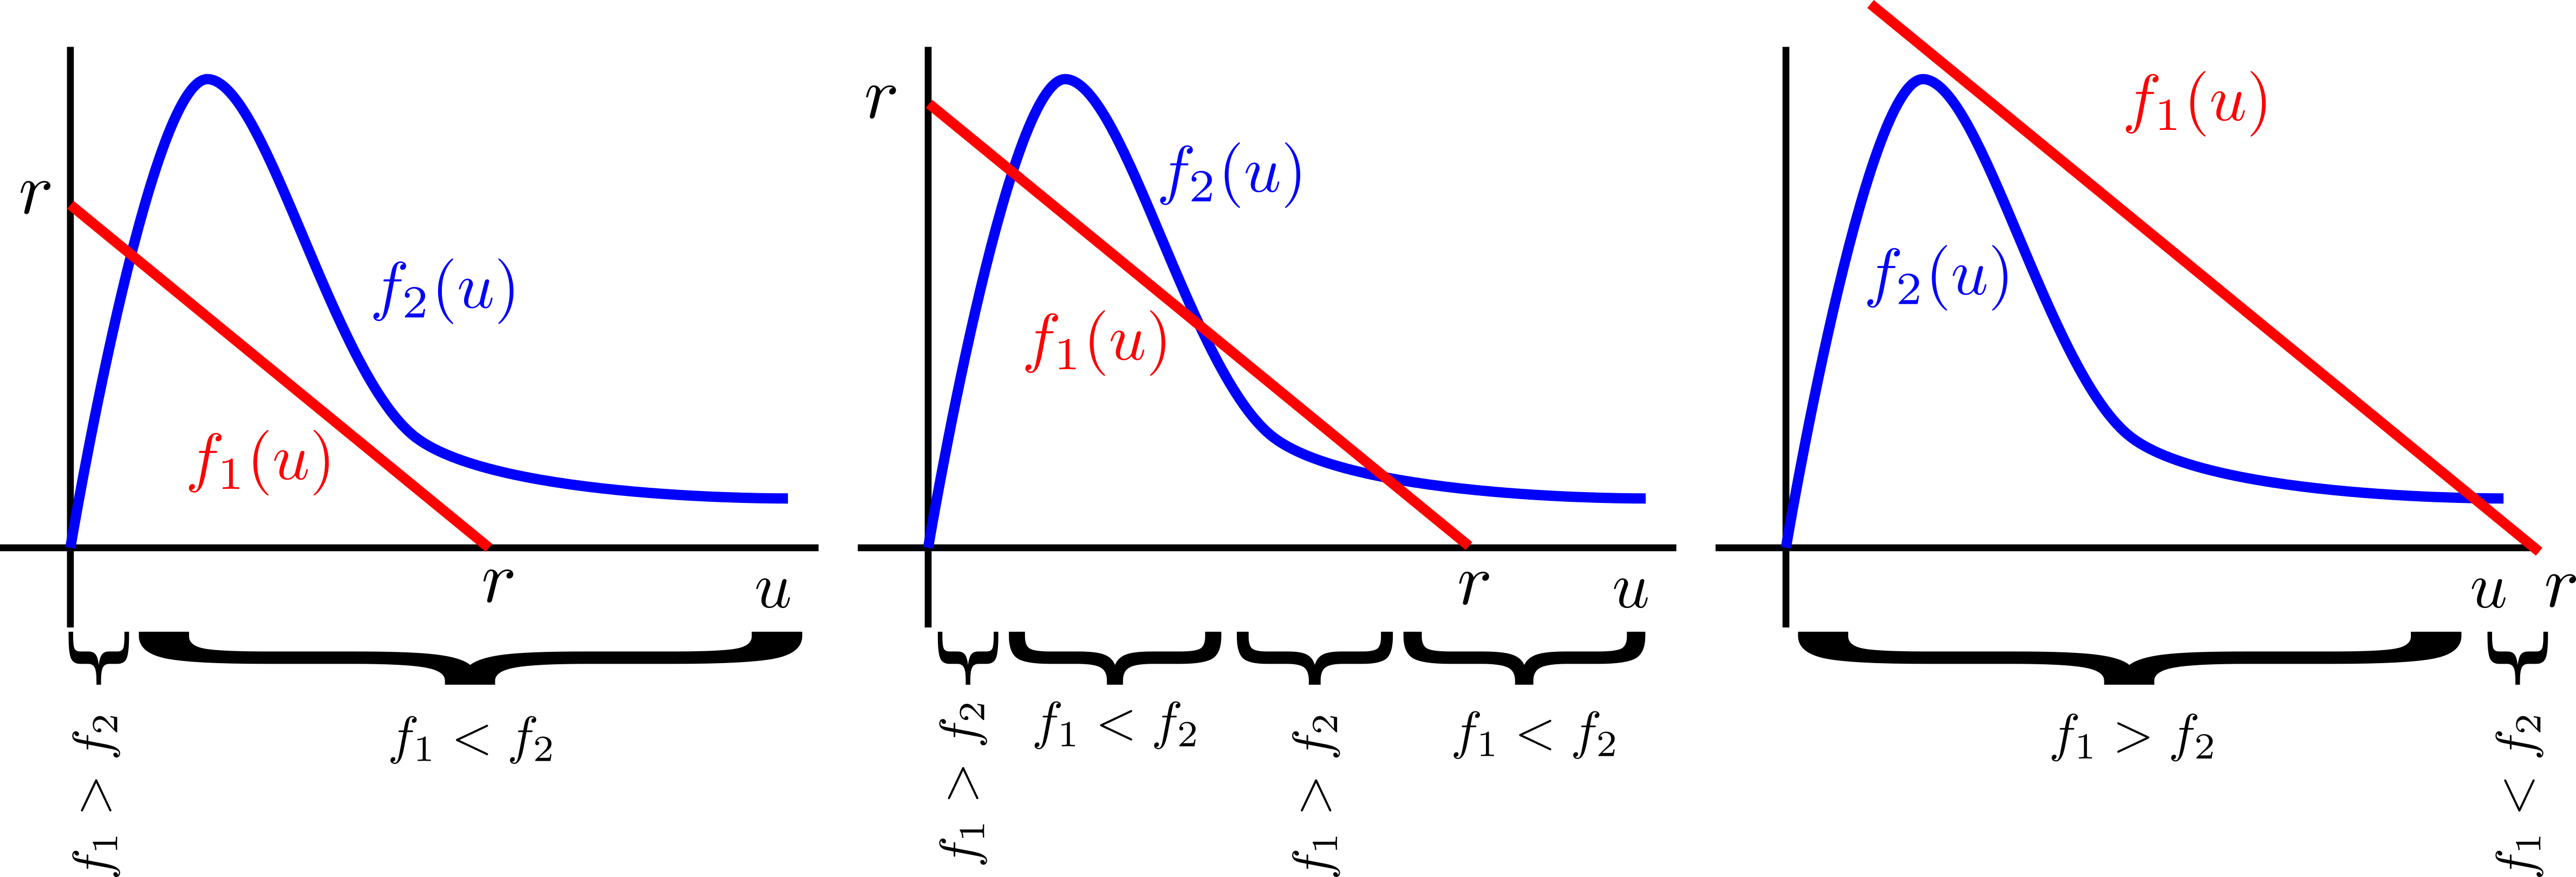
\includegraphics[width=\textwidth]{../../Pictures/f1_f2_positivity.png}
%\caption{\label{f1_f2_positivity} Plots of $f_1$ and $f_2$, for varying $r$ and fixed $r/k$. $r$ increases left to right. The brackets along the $u$ axis delineate the regions over which $f_1>f_2$ and $f_2>f_1$.}
%\end{figure}
%\subsubsection{}
%See \fig{Spruce_budworm_arrowed} for the sketches.
%\begin{figure}[h!!!]
%\centering
%\subfigure[\label{r_small_arrowed}]{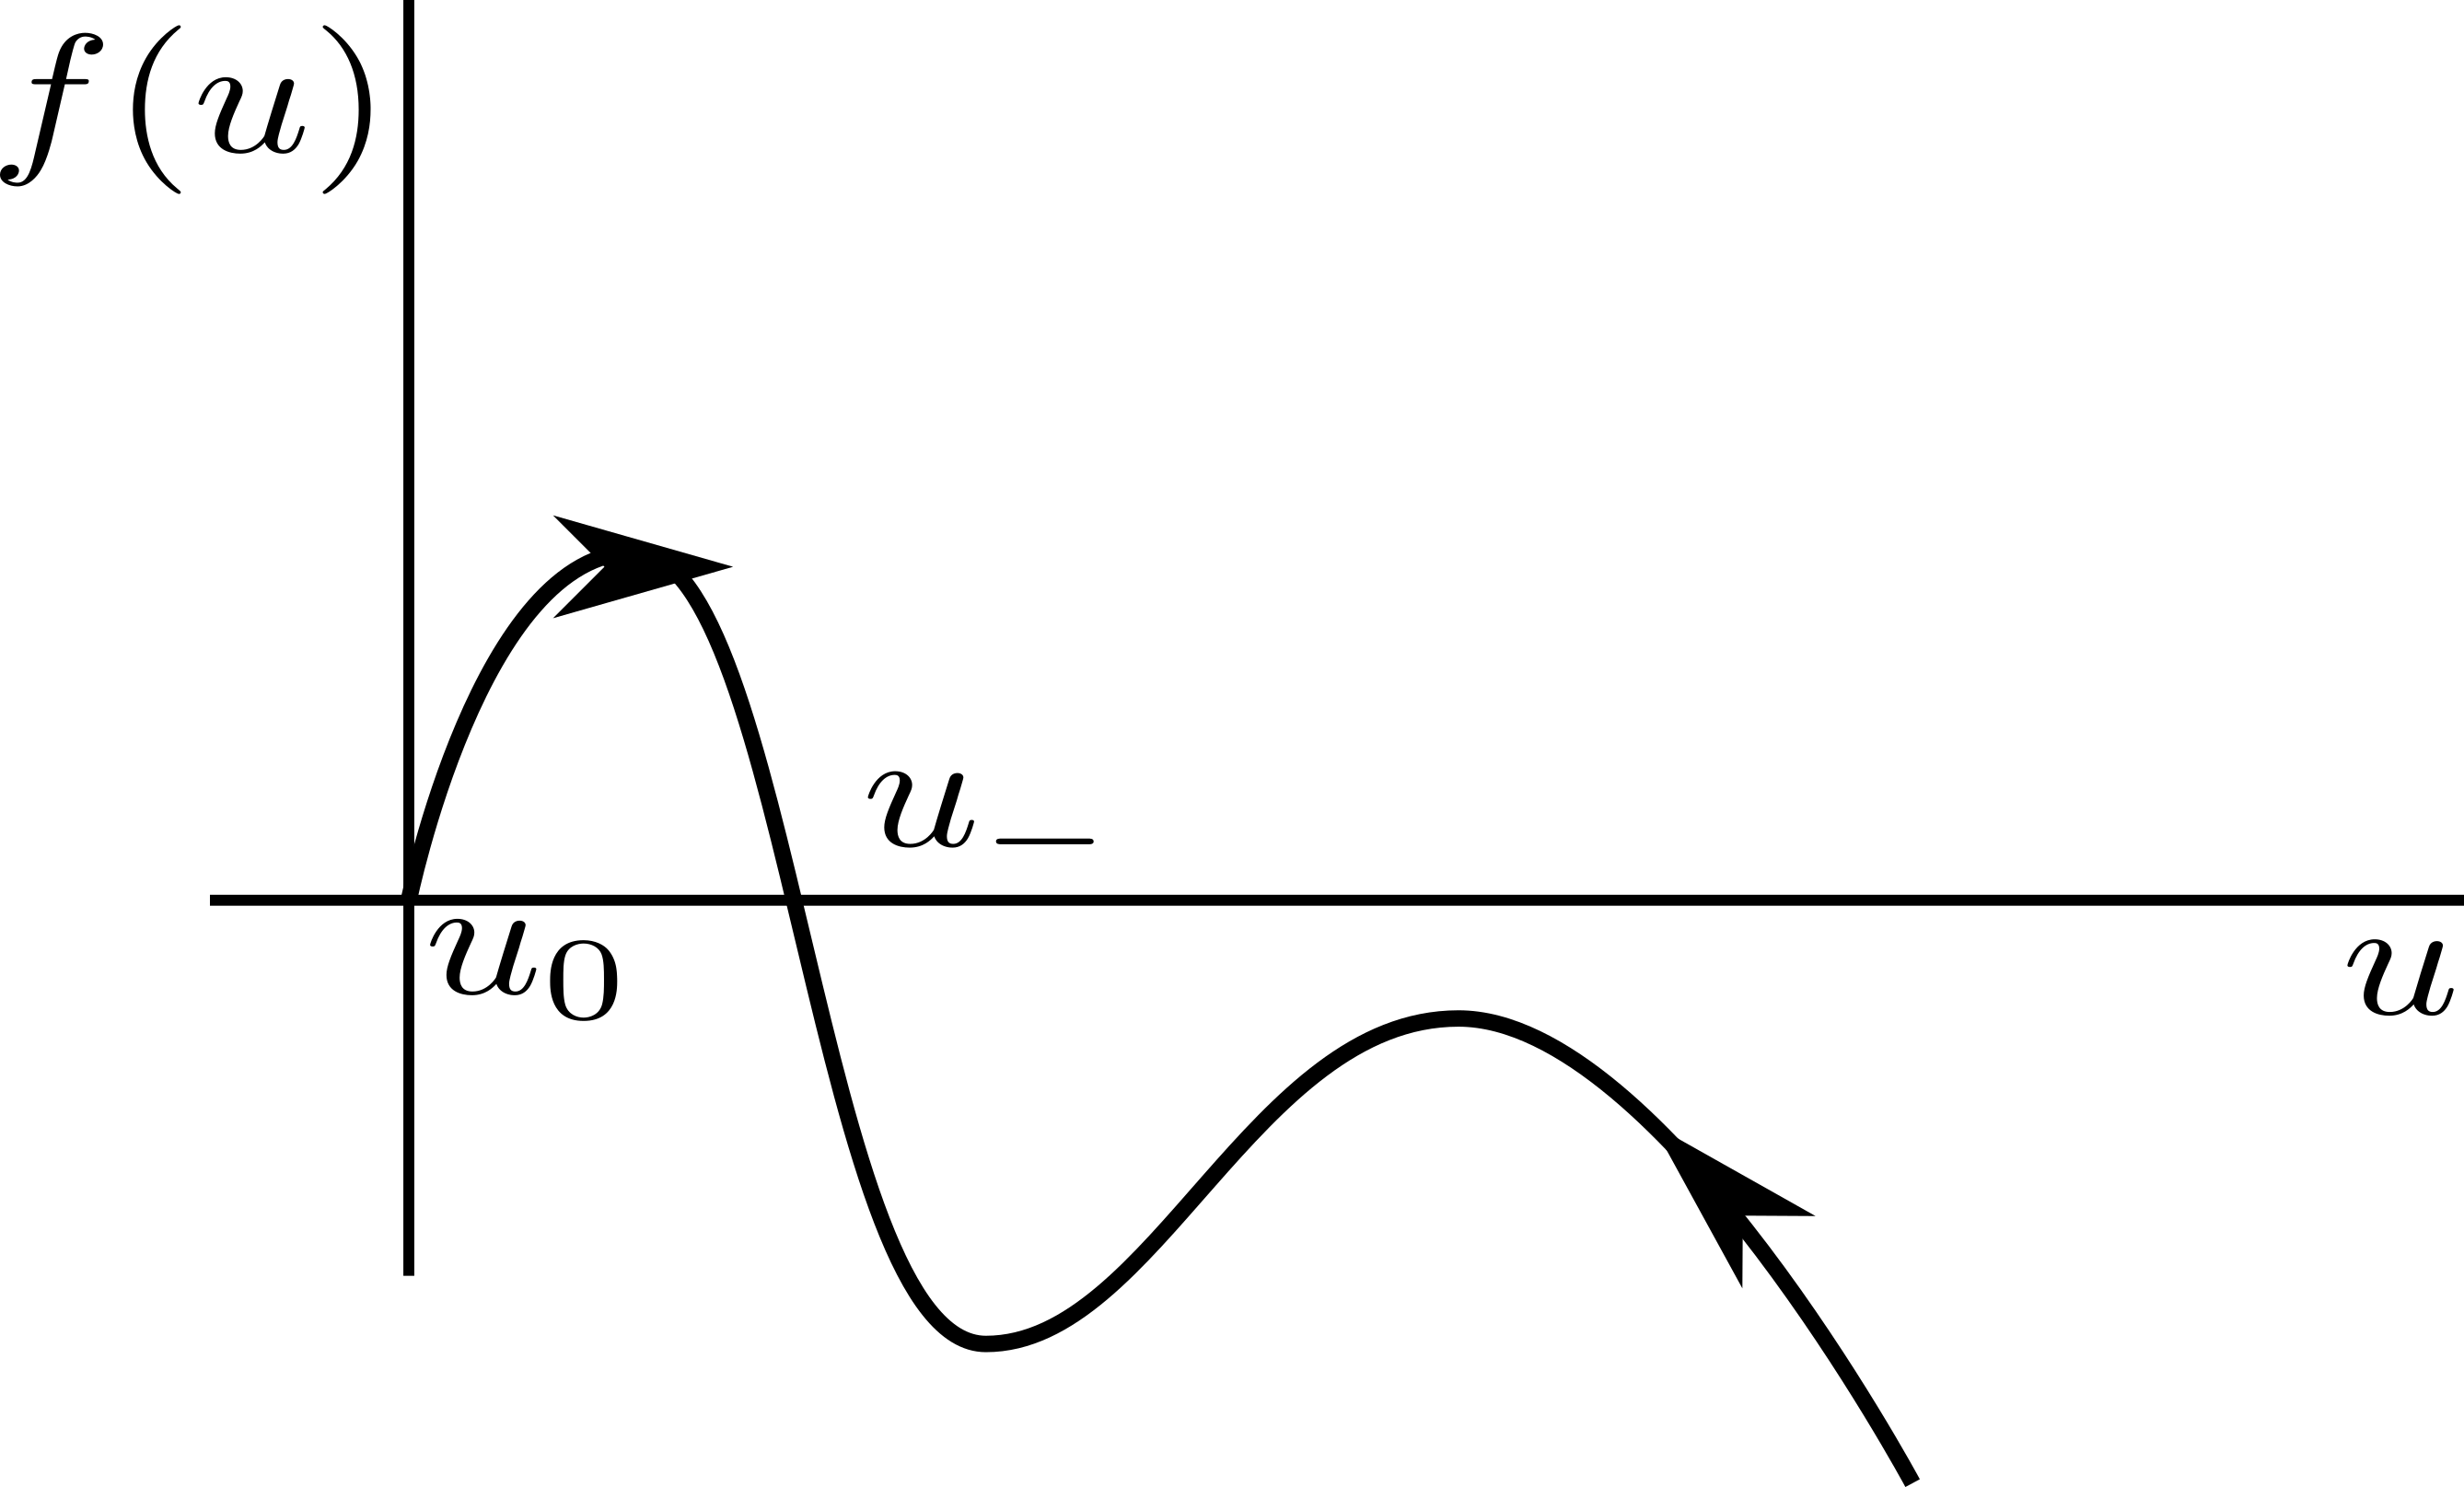
\includegraphics[width=\tttp]{../../Pictures/Spruce_budworm_r_small_arrowed.png}}
%\subfigure[\label{r_medium_arrowed}]{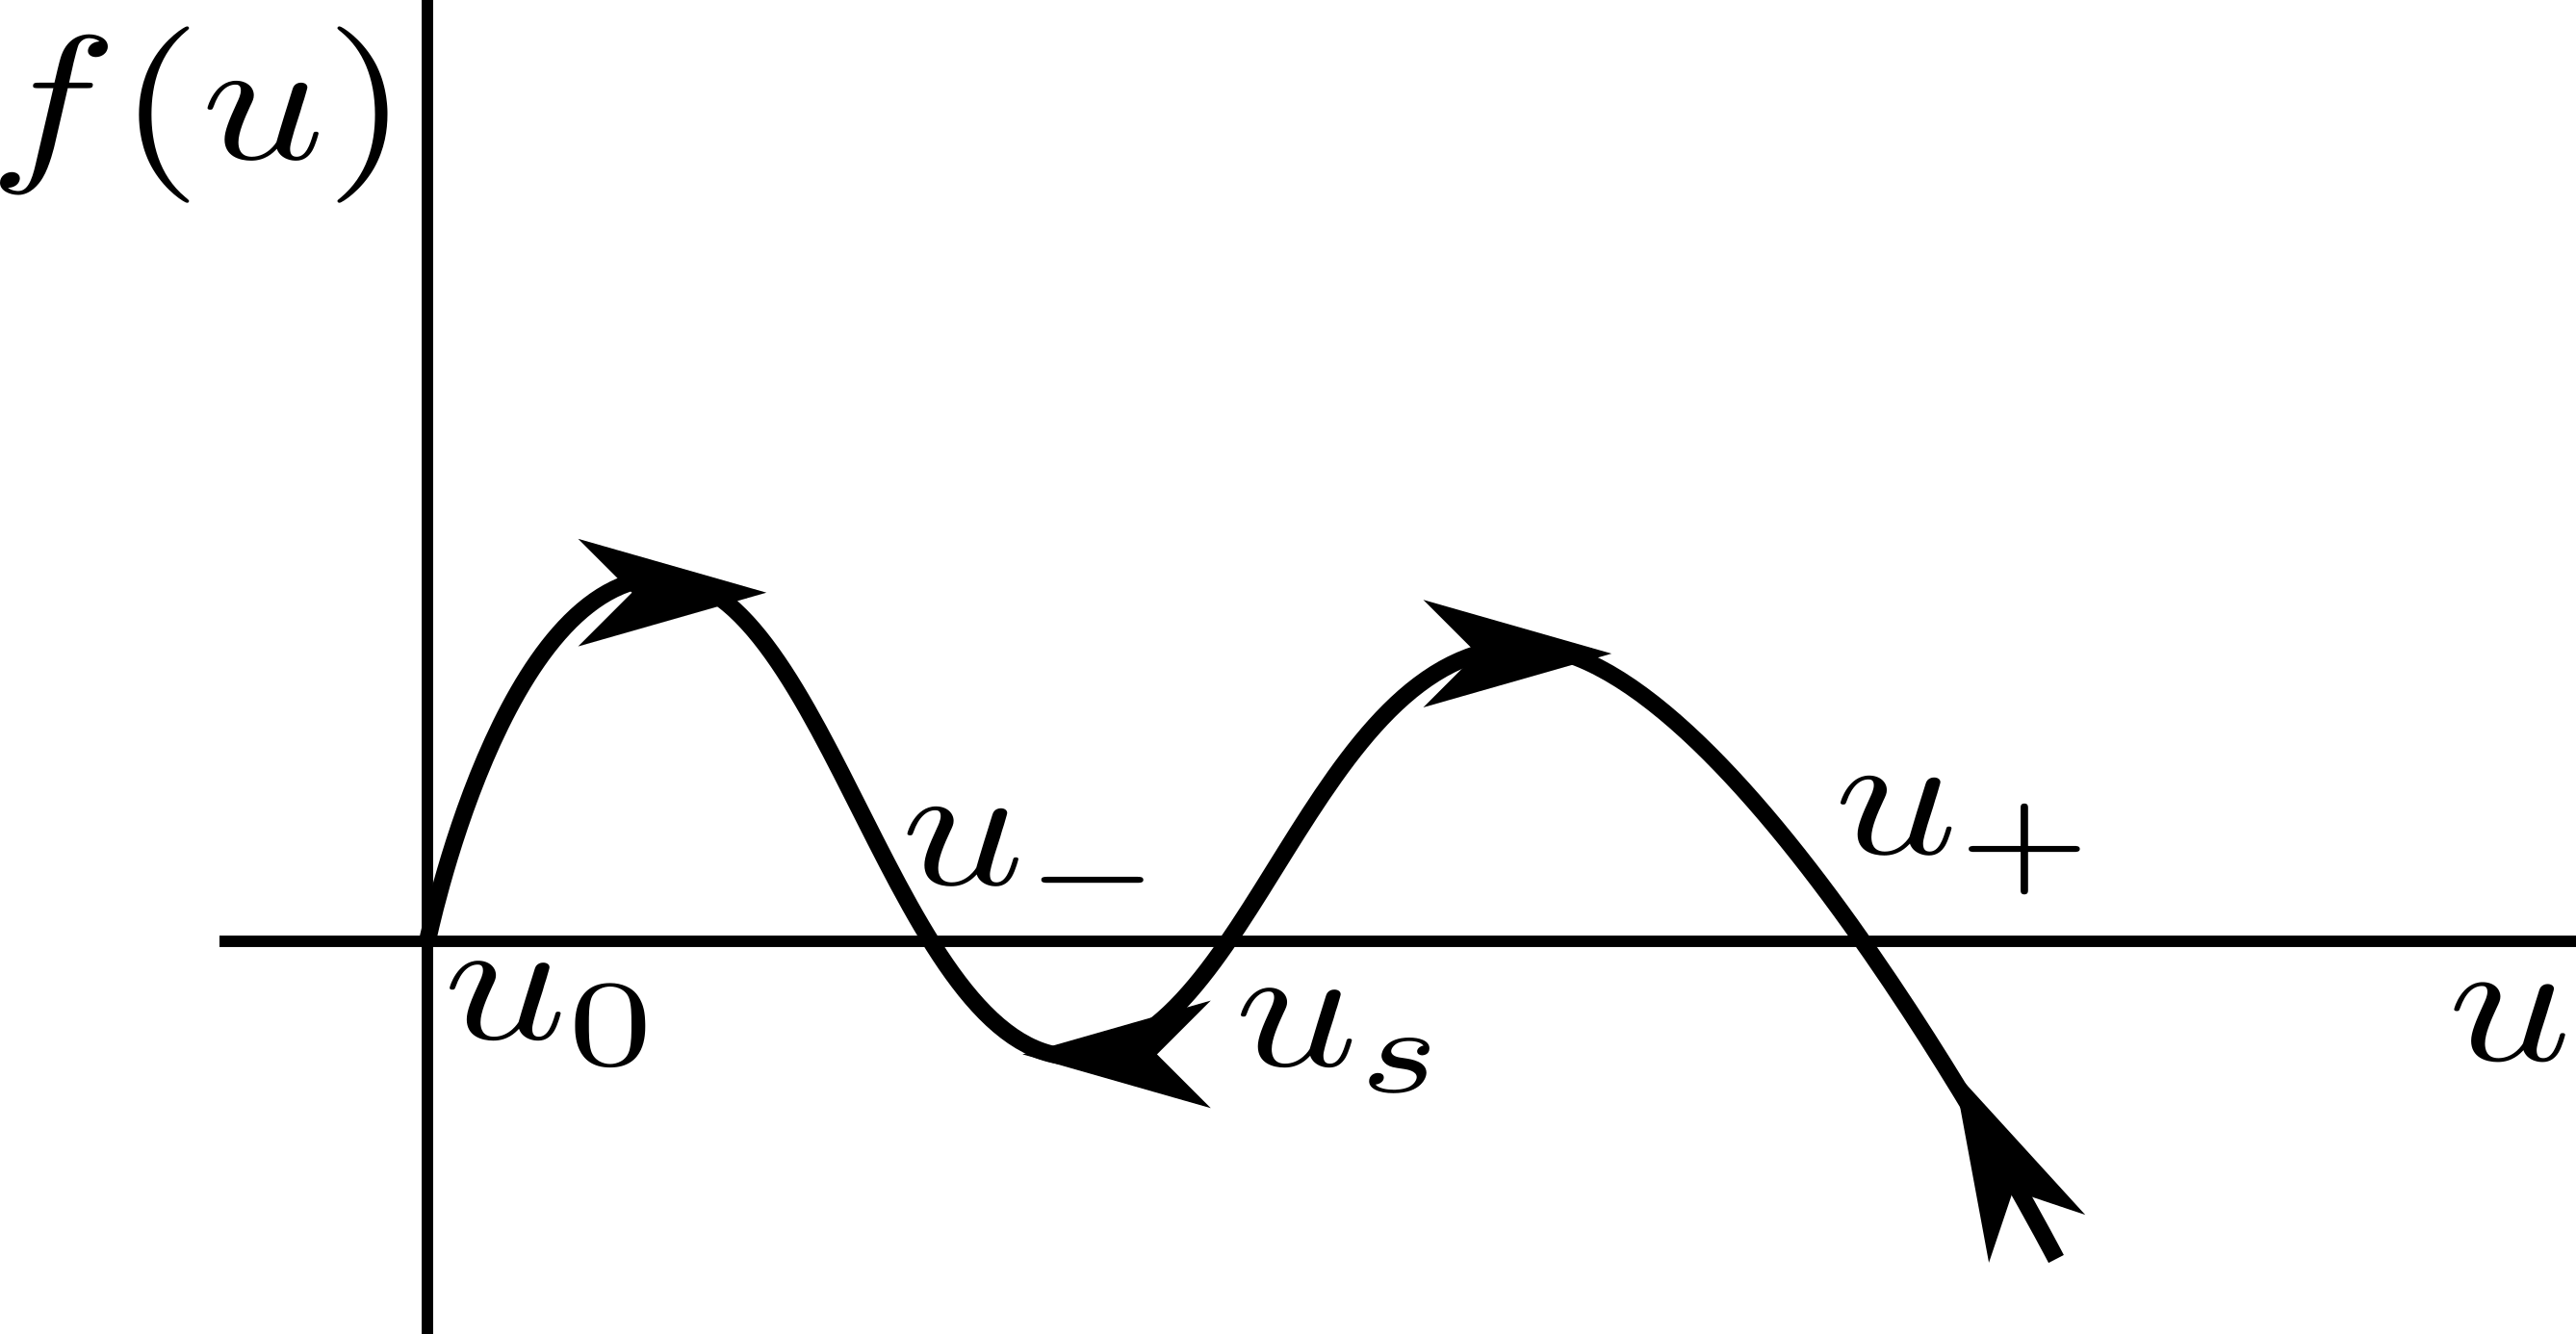
\includegraphics[width=\tttp]{../../Pictures/Spruce_budworm_r_medium_arrowed.png}}
%\subfigure[\label{r_large_arrowed}]{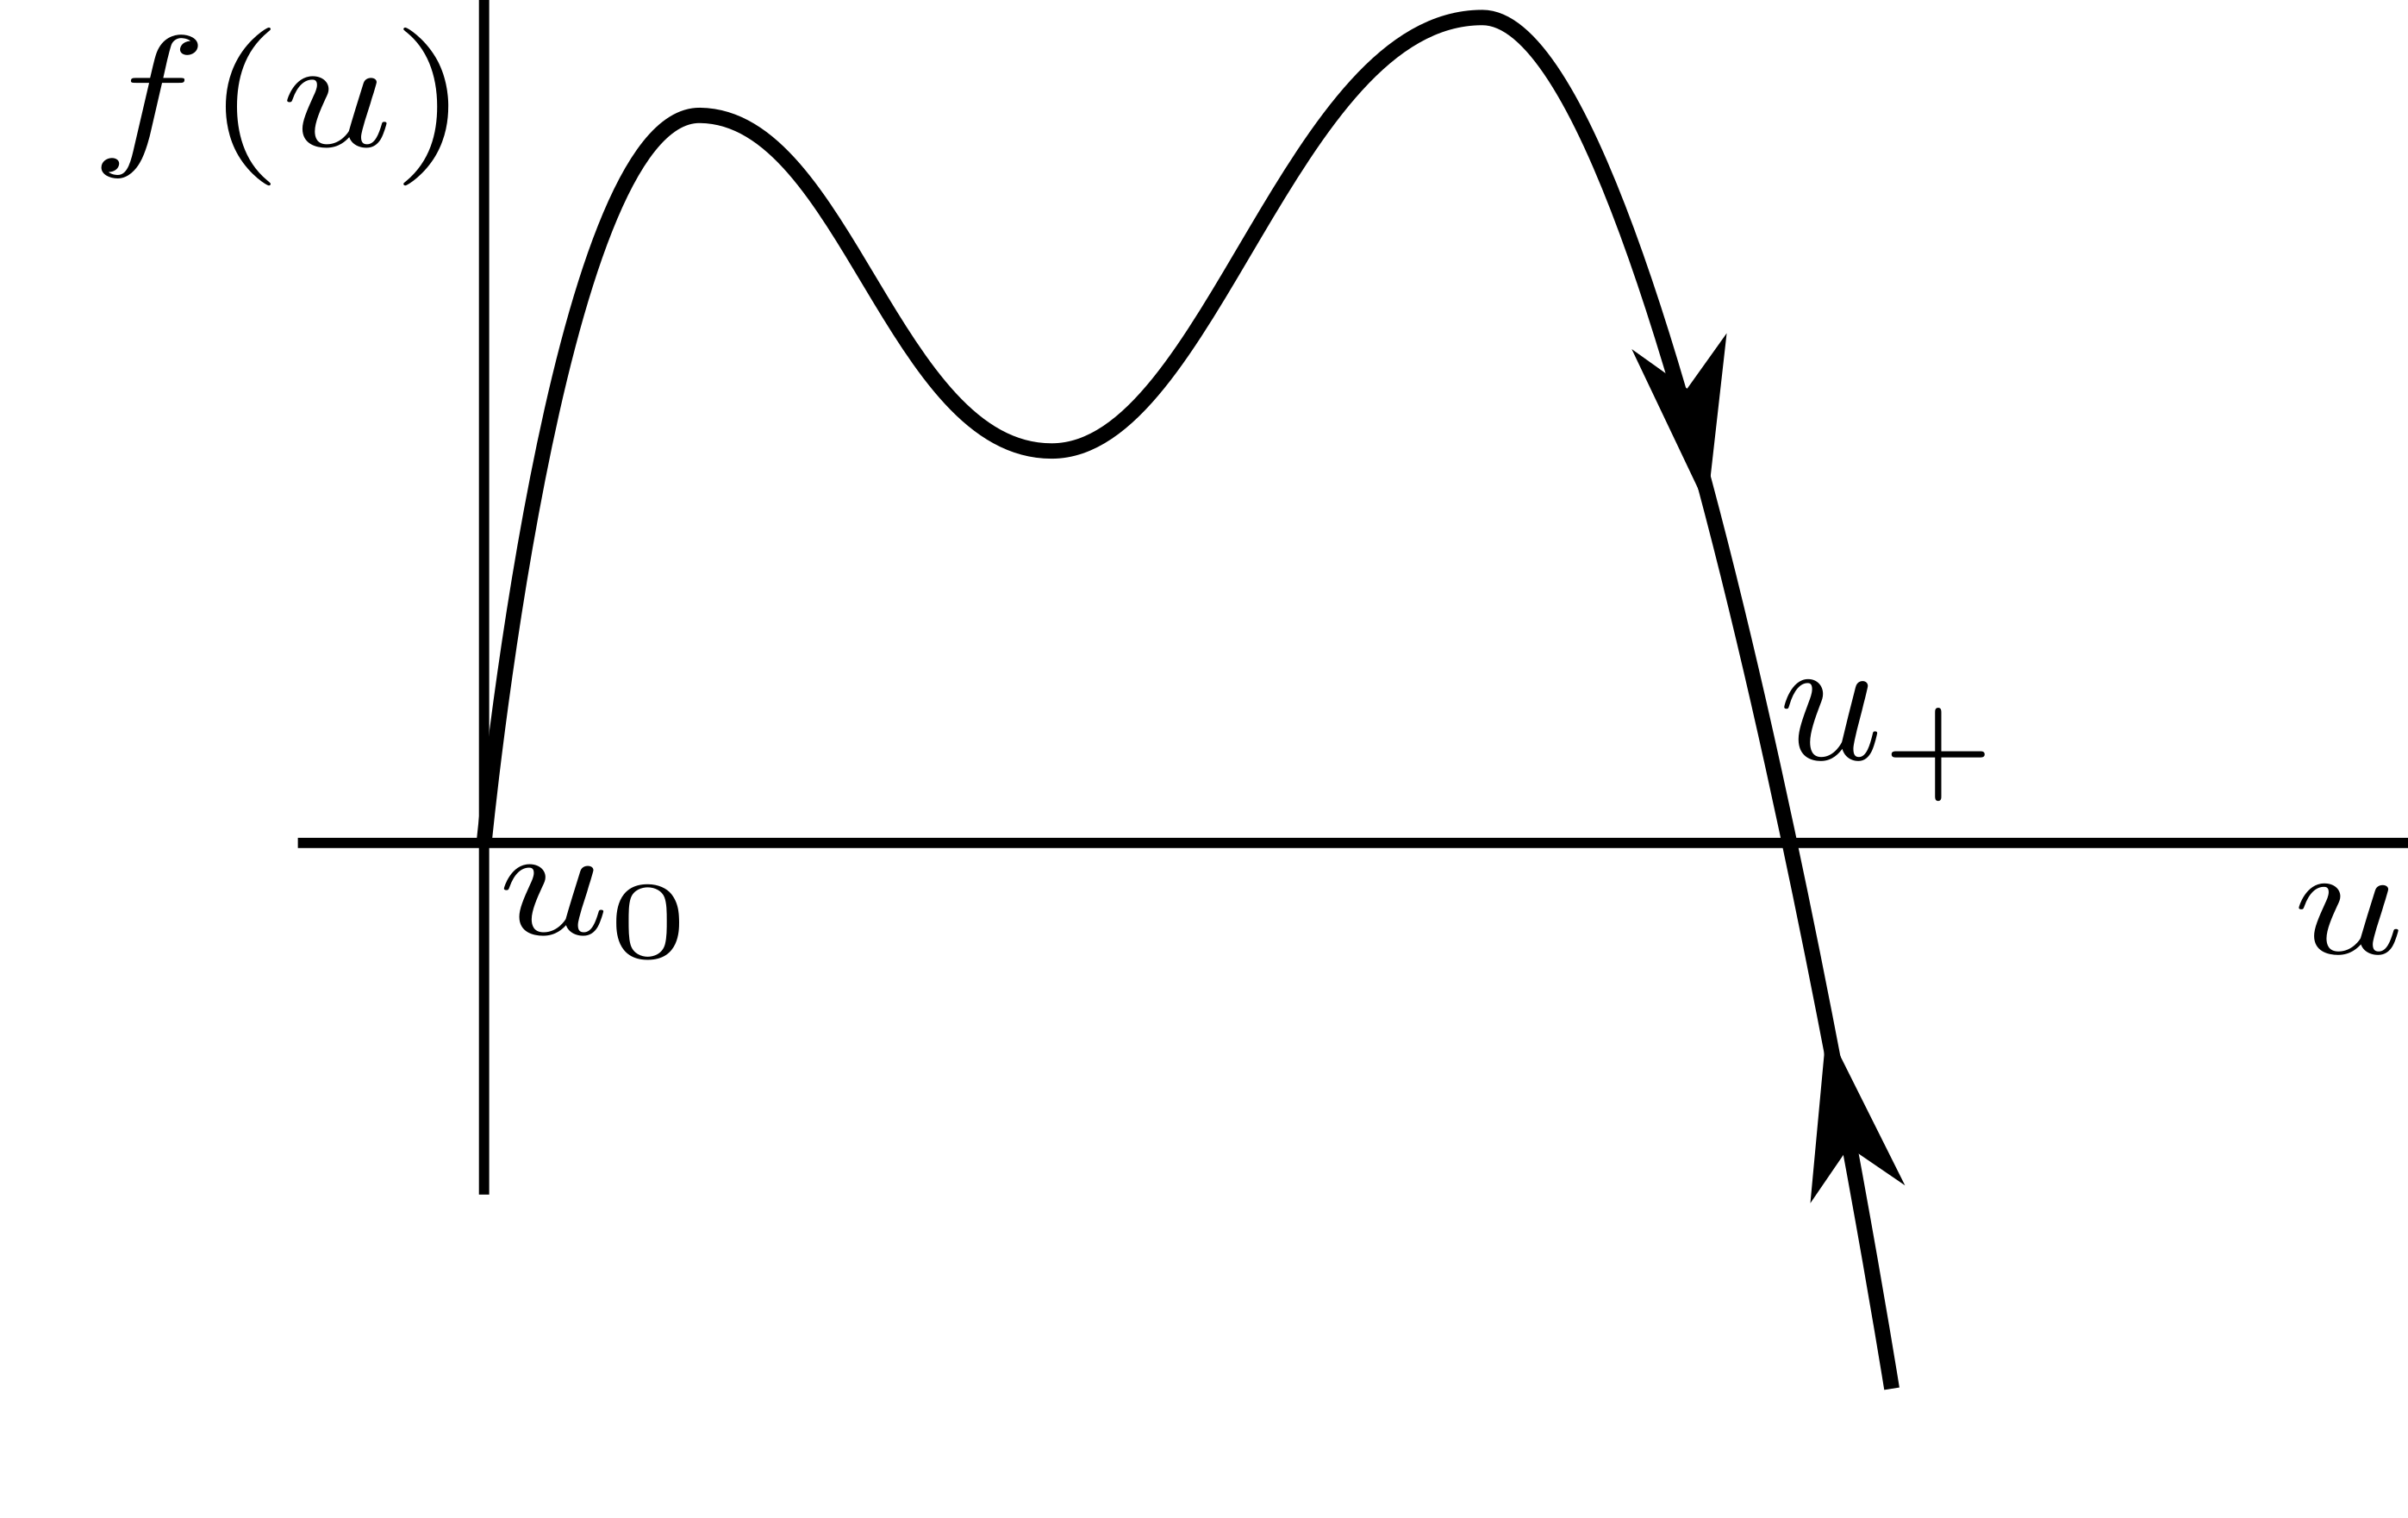
\includegraphics[width=\tttp]{../../Pictures/Spruce_budworm_r_large_arrowed.png}}
%\caption{\label{Spruce_budworm_arrowed} Three potential sketches of the spruce budworm phase plane depending on the parameter $r$, with fixed $r/k$. $r$ increases left to right.}
%\end{figure}
%\subsubsection{}
%The steady states have been specified on \fig{Spruce_budworm_arrowed}.
%\subsubsection{}
%Using \fig{Spruce_budworm_arrowed} $u_0$ is always unstable and always exists. $u_-$ and $u_+$ are always stable when they exist. $u_s$ is always unstable when it exists.
%\subsubsection{}
%\begin{enumerate}[(a)]
%\item when $r$ is small only $u_0$ and $u_-$ exist and, so, the system will tend to $u_-$.
%\item as $r$ increase $u_s$ and $u_+$ will appear, but $u_-$ is still stable and so the system stays where it is, as $u_-$.
%\item for large $r$ $u_-$ disappears. The system then evolves to $u_+$.
%\item reducing $r$ to the previous value brings back $u_-$, but $u_+$ still exists and is stable so the system stays at $u_+$.
%\item originally we were at $u_-$ now we are at $u_+$, even though we have reduced $r$ back to the previous position. Since these are different steady states the model presents hysteresis.
%\end{enumerate} 
%
%\section*{Exam revision}
%\section{Stability of a one variable system}
%Consider the following equation
%\bb
%\dot{u}=u(1-u)^3(u-2)^2(3-u)(4-u).\label{Stability_test}
%\ee
%\begin{enumerate}
%\item What are the steady states?
%\item Linearise around each steady state. Which steady states are stable and which are unstable? Why can you not categorise the stability of $u=1$ and $u=2$?
%\item Sketch the phase plane $(u,\dot{u})$ and show that your linear analysis tallies with the stability information gained from the sketch.
%\item Use the sketch to categorise the stability of $u=1$ and $u=2$.
%\end{enumerate}
%\subsection{Answer}
%\subsubsection{}
%Steady states are $u_s=0,1,2,3,4$.
%\subsubsection{}
%For linear stability analysis we need to check the sign of $\rd f(u_s)/\rd u$.
%\bb
%\frac{\rd f}{\rd u}=-2(u-1)^2(u-2)(4u^4-33u^3+88u^2-80u+12).
%\ee
%and, so,
%\begin{align}
%\frac{\rd f}{\rd u}(0)&=48>0\nonumber\\
%\frac{\rd f}{\rd u}(1)&=0\nonumber\\
%\frac{\rd f}{\rd u}(2)&=0\nonumber\\
%\frac{\rd f}{\rd u}(3)&=24>0\nonumber\\
%\frac{\rd f}{\rd u}(4)&=-432<0\nonumber.
%\end{align}
%Thus, $u_s=0,3$ are unstable, $u_s=4$ is stable and we can not categorise $u_s=1,2$ because the equation has at least a double root at these points and, as such, the derivative evaluates to zero.
%\subsubsection{}
%\fig{Revision_stability_one_variable} illustrates that $u_s=0,2,3$ are unstable, whilst $u_s=1,4$ are stable.
%\begin{figure}[h!!!tb]
%\centering
%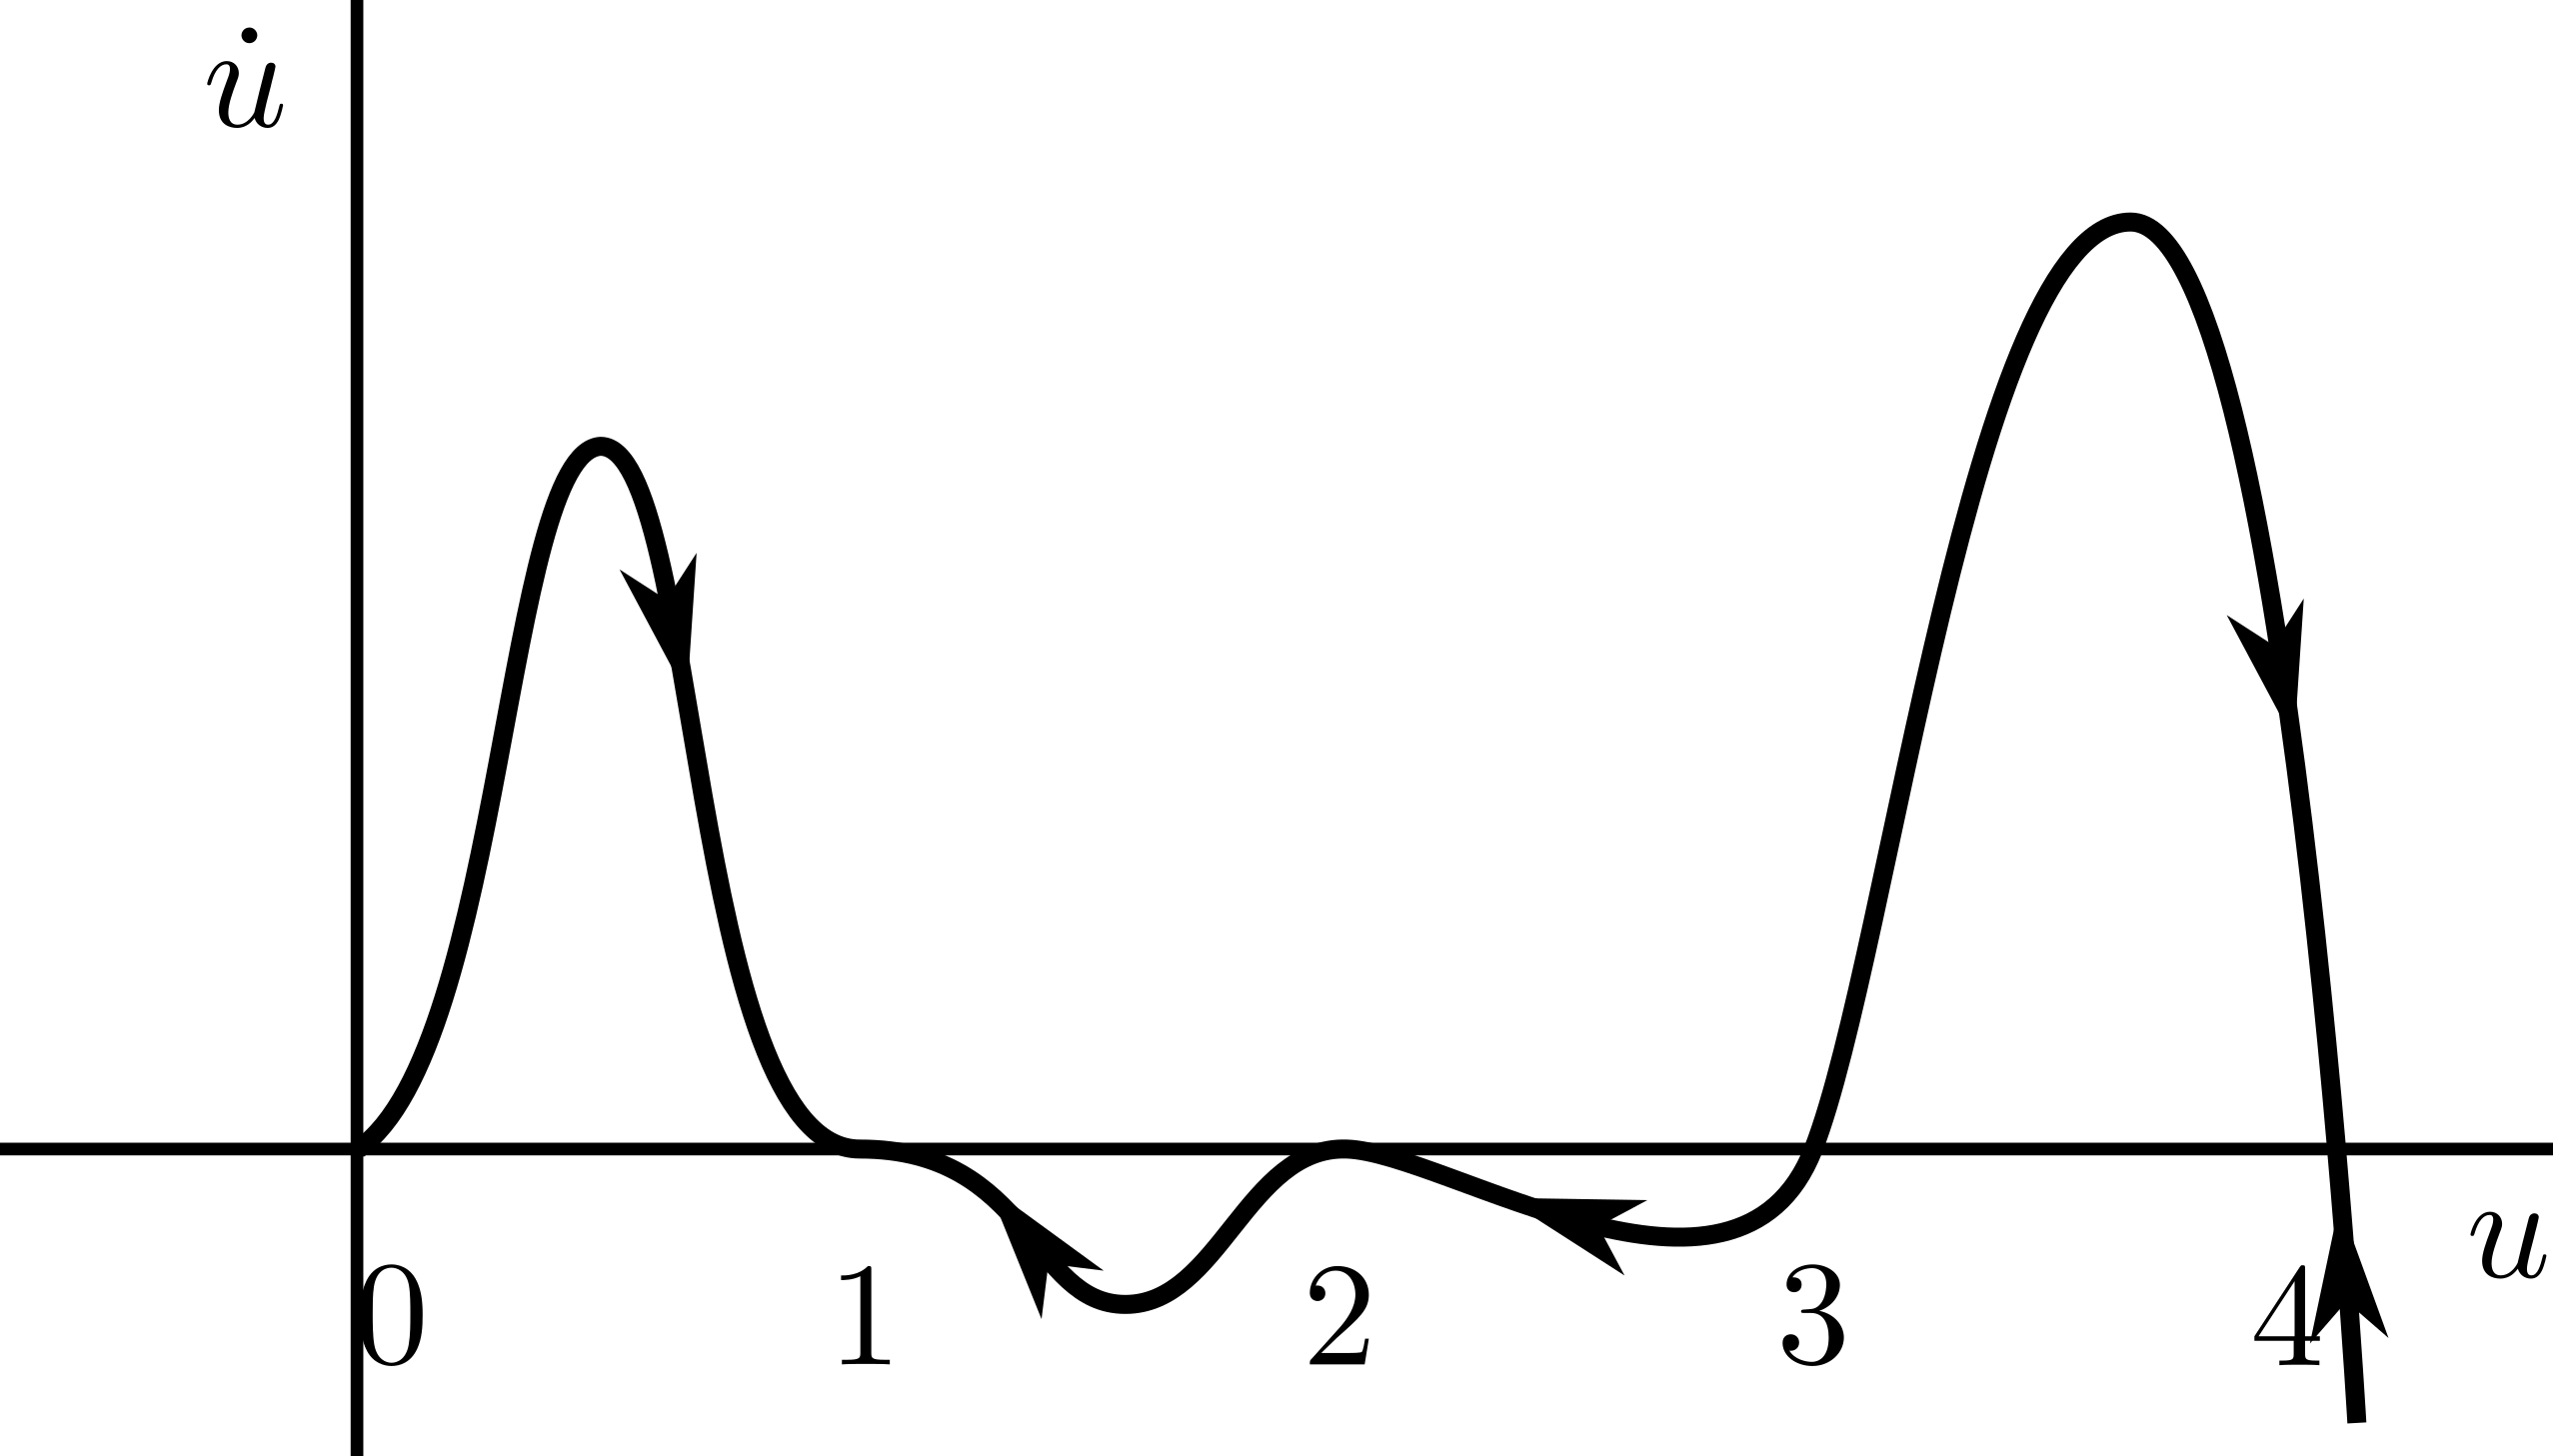
\includegraphics[width=\ttp]{../../Pictures/Revision_stability_one_variable.png}
%\caption{\label{Revision_stability_one_variable} Phase plane plot of \eqn{Stability_test}.}
%\end{figure}
%
%\section{Infections}\label{Infections}
%The interaction dynamics of any disease can be understood by modelling three sections of the population: the susceptible population, $S$; the infected population, $I$ and the recovered population, $R$. The interact through the following rules:
%\begin{itemize}
%\item whenever a susceptible agent interacts with an infective agent the result is two infective agents at a rate $r_1$;
%\item the infected population recovers at a rate proportional the size of the infected population, the rate of proportionality is $r_2$.
%\end{itemize}
%Finally, suppose that the initial densities of the susceptible and infectives are $S_0$ and $I_0$, respectively, and that there are no initially recovered people.
%\begin{enumerate}
%\item Convert the above rules into interaction equations.
%\item Use the Law of Mass Action to convert the interaction equations into ODEs.
%%of the form
%%\begin{align}
%%\dot{S}&=-r_1SI,\quad S(0)=S_0,\nonumber\\
%%\dot{I}&=r_1SI-r_2I,\quad I(0)=I_0,\nonumber\\
%%\dot{R}&=r_2I,\quad R(0)=0.
%%\end{align}
%\item Show that $S+I+R=$ constant $=S_0+I_0$. What does this mean?
%\item What are the dimensions of $S$, $I$, $R$, $\dot{S}$, $\dot{I}$, $\dot{R}$, $r_1$ and $r_2$ in terms of density and time?
%\item Let $S=[S]S'$, $I=[I]I'$, $R=[R]R'$ and $t=[t]t'$ where the bracketed variable is the dimensional part and the primed variable be the non-dimensional part. Further, suppose  we non-dimensionalise the system as
%\begin{align}
%\dot{S'}&=S'I',\quad S'(0)=S'_0,\nonumber\\
%\dot{I'}&=S'I'-I',\quad I'(0)=I'_0,\nonumber\\
%\dot{R'}&=I',\quad R'(0)=0,\nonumber
%\end{align}
%where the $\dot{}$ symbol now stands for $\rd/\rd t'$. What are the scales $[S]$, $[I]$, $[R]$ and $[t]$ in terms of $r_1$ and $r_2$? Show that they have the right dimension, \ie $[S]$ has the same dimension as $S$, as specified in question 4.
%\item What are the forms of $S'_0$ and $I'_0$ in terms of $r_1$, $r_2$, $S_0$ and $I_0$?
%\item By integrating
%\bb
%\frac{\rd I'}{\rd S'}=\frac{\dot{I}'}{\dot{S}'},\quad \frac{\rd R'}{\rd S'}=\frac{\dot{R}'}{\dot{S}'},
%\ee
%find expressions for $I'(S)$ and $R'(S)$. Do not forget about the initial conditions.
%\end{enumerate}
%\subsection{Answers}
%\subsubsection{}
%\begin{align}
%S+I&\stackrel{r_1}{\rightarrow}2I,\\
%I&\stackrel{r_2}{\rightarrow}R.
%\end{align}
%\subsubsection{}
%\begin{align}
%\dot{S}&=-r_1SI,\quad S(0)=S_0,\label{S}\\
%\dot{I}&=r_1SI-r_2I,\quad I(0)=I_0,\label{I}\\
%\dot{R}&=r_2I,\quad R(0)=0.\label{R}
%\end{align}
%\subsubsection{}
%Adding \eqnto{S}{R} we get $\rd \l S+I+R \r/\rd t=0$. Integrating and using the initial conditions produces the result $S+I+R=S_0+I_0$. This means that the total number of humans is conserved, namely they are either susceptible, infected, or removed. There is no leakage from the system.
%\subsubsection{}
%dim($S$)=dim($I$)=dim($R$)=density.
%
%\noindent dim($\dot{S}$)=dim($\dot{I}$)=dim($\dot{R}$)=density/time.
%
%\noindent dim($r_1$)=1/(density$\times$time).
%
%\noindent dim($r_2$)=1/time.
%\subsubsection{}
%Substituting $S=[S]S'$, $I=[I]I'$, $R=[R]R'$ and $t=[t]t'$, into the system we find that 
%\begin{align}
%\frac{[S]}{[t]}&=r_1[S][I],\\
%\frac{[I]}{[t]}&=r_1[S][I]=r_2[I],\\
%\frac{[R]}{[t]}&=r_2[I],
%\end{align}
%from which we rapidly find that $[S]=[I]=[R]=r_2/r_1$ and $[t]=1/r_2$. Using the results from question 4 we find that $r_2/r_1=$density and $1/r_2=$time. Thus, units are consistent.
%\subsubsection{}
%$S'_0=S_0/[S]=r_1S_0/r_2.$\\
%$I'_0=I_0/[I]=r_1I_0/r_2.$
%
%\subsubsection{}
%\begin{align}
%\frac{\rd I'}{\rd S'}=\frac{\dot{I'}}{\dot{S'}}&=1-\frac{1}{S'},\nonumber\\
%\frac{\rd R'}{\rd S'}=\frac{\dot{R'}}{\dot{S'}}&=\frac{1}{S'},\nonumber
%\end{align}
%Integrating the above equations with initial conditions $I'(S'_0)=I'_0$ gives
%\bb
%I'(S') = \log\l \frac{S'}{S'_0}\r+I'_0+S'-S'_0.
%\ee
%and
%\bb
%R'=\log\l \frac{S'}{S'_0}\r.
%\ee
\end{document}